% !TEX program = pdflatex
% !TEX encoding = UTF-8 Unicode
% !TEX spellcheck = en-US
% !BIB program = biber

%%
 % Copyright (C) 2017, Samuel Ivan Gunadi.
 % All rights reserved.
 %%

\documentclass[a4paper, 12pt, oneside]{book}

% language
\usepackage[american]{babel}

% encoding
\usepackage[T1]{fontenc}
% for non utf8 engine
\usepackage[utf8]{inputenc}

% document dimensions
\usepackage[top = 1.58 in, bottom = 1.18 in, left = 1.58 in, right = 1.18 in]{geometry}

% bibliography
% dashed=false removes dash if the authors are the same
\usepackage[backend=biber, style=ieee, language=auto, dashed=false]{biblatex}

% fonts
\usepackage{times}
\usepackage{inconsolata}
% OpenType Unicode maths fonts
\usepackage[notextcomp]{stix}

% colors
\usepackage[table]{xcolor}

% space between lines
\usepackage{setspace}

% ams packages
\usepackage{amsmath}
\usepackage{amsthm}
% \usepackage{amssymb} % use stix

% SI units
\usepackage[binary-units=true]{siunitx}

%  Case conversion ignoring mathematics, etc
\usepackage{textcase}

% source code listings
% \usepackage{listings} % use minted now
\usepackage[newfloat]{minted}

% set options
\setminted{breaklines, breakautoindent=true, breaksymbolleft=, breaksymbolindentleft=0pt, breaksymbolsepleft=0pt, breaksymbolright=\raisebox{0ex}{\scriptsize\ensuremath{\carriagereturn}}, breaksymbolindentright=12pt, breaksymbolsepright=0pt, breakanywhere=true, fontsize=\footnotesize, frame=single, linenos}
% set style
\usemintedstyle{vs}
% customize the display style of line numbers
\renewcommand\theFancyVerbLine{\ttfamily\arabic{FancyVerbLine}}

% Reimplementation of and extensions to LaTeX verbatim
\usepackage{verbatim}

%  Place selected parts of a document in landscape
\usepackage{lscape}

% pseudocode
\usepackage{algorithm}
\usepackage{algpseudocode}

% Split long sequences of characters in a neutral way
\usepackage{seqsplit}

% images
\usepackage{graphicx}

% tables
\usepackage{array}
\usepackage{tabu}
\usepackage{multirow}

% title styles
\usepackage{titlesec}
\usepackage{titletoc}

% headers and footers
\usepackage{fancyhdr}

% Add bibliography/index/contents to Table of Contents
\usepackage[notbib]{tocbibind}

% customize captions in floating environments (captionof)
\usepackage{caption}

% context sensitive quotation facilities
\usepackage{csquotes}

\newenvironment{longlisting}{\captionsetup{type=listing}}{}

% hyperlink
\usepackage{hyperref}

% plots
\usepackage{pgfplots}

% appendix titles
\usepackage{appendix}

% e-TeX tools for LaTeX
\usepackage{etoolbox}

% Verbatim with URL-sensitive line breaks
\usepackage{url}

% Control layout of itemize, enumerate, description
\usepackage{enumitem}

\setlist{nosep}

\pgfplotsset{compat=1.14}

% remove header and footer horizontal line
\renewcommand{\headrulewidth}{0pt}
\renewcommand{\footrulewidth}{0pt}

% title formatting

\renewcommand{\thechapter}{\Roman{chapter}}
\renewcommand{\thesection}{\arabic{chapter}.\arabic{section}}
\renewcommand{\thefigure}{\arabic{chapter}.\arabic{figure}}
\renewcommand{\thetable}{\arabic{chapter}.\arabic{table}}
\renewcommand{\theequation}{\arabic{chapter}.\arabic{equation}}
\renewcommand{\thelisting}{\arabic{chapter}.\arabic{listing}}

\titlespacing*{\chapter}{0pt}{0pt}{20pt}
\titleformat
    {\chapter}
    [display]
    {\bfseries\large}
    {\centering\MakeTextUppercase{\chaptertitlename}~\thechapter}
    {0ex}
    {
        \centering\MakeTextUppercase
    }
    [
    ]
\titleformat*{\section}{\bfseries\normalsize}
\titleformat*{\subsection}{\bfseries\normalsize}
\titleformat*{\subsubsection}{\bfseries\normalsize}

% table of contents formatting

\titlecontents{chapter}
[0em] % left-margin
{} % above-code
{\bfseries\MakeTextUppercase{\chaporappname}\ \thecontentslabel\quad} % numbered-format
{\bfseries} % unnumbered-format
{\hfill\contentspage} % filler-page-format

\let\chaporappname\chaptername

% change the name of certain headings
\addto\captionsamerican{
    \renewcommand{\contentsname}{TABLE OF CONTENTS}
    %\renewcommand{\bibname}{BIBLIOGRAPHY}
    \renewcommand{\listfigurename}{LIST OF FIGURES}
    \renewcommand{\listtablename}{LIST OF TABLES}
    \renewcommand{\listlistingname}{LIST OF LISTINGS}
    \renewcommand{\appendixname}{APPENDIX}
}

% bibliography file
\addbibresource{bibliography.bib}

% line breaking rules
\emergencystretch 3em

% define custom "parallel for" for algorithmicx package
\algblockdefx{ParallelFor}{EndParallelFor}[1]
    {\textbf{for }#1 \textbf{do in parallel}}
    {\textbf{end for}}


\begin{document}

\frontmatter

%%
 % Title page
 %%
 
\thispagestyle{empty}
\addcontentsline{toc}{chapter}{TITLE PAGE}

\begin{center}
    \begin{doublespace}
        
        \textbf{\MakeTextUppercase{Thesis}}
        
        \bigskip
        
        {\bfseries\large\MakeTextUppercase{Real-Time GPU-Based SPH Fluid Simulation Using Vulkan and OpenGL Compute Shaders}}
        
        \bigskip
        % UPH format: the word "part" in this case is a mass noun; "a part" is incorrect
        \small{submitted in partial fulfillment of the requirements for the degree of\par Sarjana Informatika Strata Satu}
        
        \vspace{1.5cm}
        
        \textbf{by}
        
        \begin{tabular}{>{\bfseries}l >{\bfseries}l}
            \MakeTextUppercase{Name} & \MakeTextUppercase{: Samuel Ivan Gunadi} \\
            \MakeTextUppercase{Student ID} & \MakeTextUppercase{: 11220120018}
        \end{tabular}
        
        \vspace{3cm}
        
    \end{doublespace}
    \includegraphics[height=4cm, width=4cm]{images/uph_logo.png}
    \vspace{3.5cm}
    \begin{singlespace}
        \bfseries
        \MakeTextUppercase{Department of Informatics}
        
        \MakeTextUppercase{Faculty of Computer Science}
        
        \MakeTextUppercase{Universitas Pelita Harapan}
        
        \MakeTextUppercase{Tangerang}
        
        \MakeTextUppercase{2018}
    \end{singlespace}
\end{center}

\clearpage

% set header and footer style

\pagestyle{fancy}
\fancyhf{}
\fancyfoot[R]{\thepage}

% also redefine the plain style because the "\chapter" macro contains "\thispagestyle{plain}"

\fancypagestyle{plain}
{
    \fancyhf{}
    \fancyfoot[R]{\thepage}
    \renewcommand{\headrulewidth}{0pt}
    \renewcommand{\footrulewidth}{0pt}
}

%%
 % Legal 1
 %%

% Logo header
\noindent
\begin{tabu} to \linewidth {m{2.5cm} >{\setlength{\baselineskip}{2\baselineskip}}X[m]}
    \includegraphics[width=2.2cm, height=2.2cm]{images/uph_logo.png} & \textbf{\Large UNIVERSITAS PELITA HARAPAN \newline FAKULTAS ILMU KOMPUTER} \\
\end{tabu}

\noindent\rule{\textwidth}{1mm}

\begingroup
    \titlespacing*{\chapter}{0pt}{12pt}{12pt}
    \titleformat
        {\chapter}
        [display]
        {\bfseries\large}
        {\centering}
        {0ex}
        {
            \centering\MakeTextUppercase
        }
        [
        ]
    {
        \let\clearpage\relax
        % for double sided, use \let\cleardoublepage\relax
        \chapter{PERNYATAAN KEASLIAN KARYA TUGAS AKHIR}
    }
\endgroup

\begin{onehalfspace}
    \noindent Saya, sebagai mahasiswa Teknik Informatika di Universitas Pelita Harapan,
    
    \begin{tabbing}
        \hspace{3cm}\=\textbf{Nama} \hspace{2cm}\= \textbf{: Samuel Ivan Gunadi} \\
        \>\textbf{NIM} \> \textbf{: 11220120018} \\
        \>\textbf{Program Studi} \> \textbf{: Teknik Informatika} \\
        \>\textbf{Konsentrasi} \> \textbf{: Rekayasa Piranti Lunak}
    \end{tabbing}
    
    \noindent menyatakan bahwa karya tugas akhir yang saya buat dengan judul {\bfseries\MakeTextUppercase{Real-Time GPU-Based SPH Fluid Simulation Using Vulkan and OpenGL Compute Shaders}}:
    
    \begin{enumerate}
        \item dibuat dan diselesaikan sendiri, dengan menggunakan hasil kuliah, tinjauan lapangan dan buku-buku serta jurnal acuan yang tertera di dalam referensi pada karya tugas akhir saya,
        \item bukan merupakan duplikasi karya tulis yang sudah dipublikasikan atau yang pernah dipakai untuk mendapatkan gelar sarjana di universitas lain, kecuali pada bagian-bagian sumber informasi dicantumkan dengan cara referensi yang semestinya, dan
        \item bukan merupakan karya terjemahan dari kumpulan buku atau jurnal acuan yang tertera di dalam referensi pada karya tugas akhir saya.
    \end{enumerate}
    \noindent Kalau terbukti saya tidak memenuhi apa yang telah dinyatakan di atas, maka karya tugas akhir ini batal.
    \begin{flushright}
        Tangerang, 8 Januari 2018
        
        Yang membuat pernyataan
        
        \vspace{3\baselineskip}
        Samuel Ivan Gunadi
    \end{flushright}
\end{onehalfspace}
\clearpage

%%
 % Legal 2
 %%

%% Logo header
\noindent
\begin{tabu} to \linewidth {m{2.5cm} >{\setlength{\baselineskip}{2\baselineskip}}X[m]}
    \includegraphics[width=2.2cm, height=2.2cm]{images/uph_logo.png} & {\bfseries\Large UNIVERSITAS PELITA HARAPAN \newline FAKULTAS ILMU KOMPUTER} \\
\end{tabu}
\noindent\rule{\textwidth}{1mm}

\begingroup
    \titlespacing*{\chapter}{0pt}{12pt}{12pt}
    \titleformat
        {\chapter}
        [display]
        {\bfseries\large}
        {\centering}
        {0ex}
        {
            \centering\MakeTextUppercase
        }
        [
        ]
    {
        \let\clearpage\relax
        % for double sided, use \let\cleardoublepage\relax
        \chapter{PERSETUJUAN DOSEN PEMBIMBING TUGAS AKHIR}
    }
\endgroup

\begin{onehalfspace}
    \begin{center}
        {\bfseries\MakeTextUppercase{Real-Time GPU-Based SPH Fluid Simulation Using Vulkan and OpenGL Compute Shaders}}
        
        oleh
        
    \end{center}
    
    \begin{tabbing}
        \hspace{3cm}\=\textbf{Nama} \hspace{2cm}\= \textbf{: Samuel Ivan Gunadi} \\
        \>\textbf{NIM} \> \textbf{: 11220120018} \\
        \>\textbf{Program Studi} \> \textbf{: Teknik Informatika} \\
        \>\textbf{Konsentrasi} \> \textbf{: Rekayasa Piranti Lunak}
    \end{tabbing}
    telah diperiksa dan disetujui untuk diajukan dan dipertahankan dalam sidang tugas akhir guna memperoleh gelar Sarjana Informatika Strata Satu pada program studi Teknik Informatika, Fakultas Ilmu Komputer di Universitas Pelita Harapan, Tangerang, Banten.

    \begin{center}
        Tangerang, 8 Januari 2018
        
        Menyetujui:
        
        \vspace{1 cm}
        \begin{tabu} to \linewidth {p{6cm} X p{6cm}}
            \textbf{Pembimbing Utama} & & \textbf{Co-Pembimbing} \\
            \\
            \\
            \\
            Dr. Pujianto Yugopuspito & & Dr. David H. Hareva \\
            \\
            \textbf{Ketua Program Studi \newline Teknik Informatika} & & \textbf{Pembantu Dekan \newline Fakultas Ilmu Komputer} \\
            \\
            \\
            \\
            Irene A. Lazarusli, S.Kom., M.T. & & Hendra Tjahyadi, S.T., M.T., Ph.D.
        \end{tabu}
    \end{center}
\end{onehalfspace}
\clearpage

%%
 % Legal 3
 %%

% Logo header
\noindent
\begin{tabu} to \linewidth {m{2.5cm} >{\setlength{\baselineskip}{2\baselineskip}}X[m]}
    \includegraphics[width=2.2cm, height=2.2cm]{images/uph_logo.png} & \textbf{\Large UNIVERSITAS PELITA HARAPAN \newline FAKULTAS ILMU KOMPUTER} \\
\end{tabu}

\noindent\rule{\textwidth}{1mm}

\begingroup
    \titlespacing*{\chapter}{0pt}{12pt}{12pt}
    \titleformat
        {\chapter}
        [display]
        {\bfseries\large}
        {\centering}
        {0ex}
        {
            \centering\MakeTextUppercase
        }
        [
        ]
    {
        \let\clearpage\relax
        % for double sided, use \let\cleardoublepage\relax
        \chapter{PERSETUJUAN TIM PENGUJI TUGAS AKHIR}
    }
\endgroup

\begin{onehalfspace}
    \noindent Pada 30 Januari 2018 telah diselenggarakan sidang tugas akhir untuk memenuhi sebagian persyaratan akademik guna memperoleh gelar Sarjana Informatika Strata Satu pada program studi Teknik Informatika, Fakultas Ilmu Komputer, Universitas Pelita Harapan, atas nama
    
    \noindent \begin{tabbing}
    \hspace{3cm}\=\textbf{Nama} \hspace{2cm}\= \textbf{: Samuel Ivan Gunadi} \\
    \>\textbf{NIM} \> \textbf{: 11220120018} \\
    \>\textbf{Program Studi} \> \textbf{: Teknik Informatika} \\
    \>\textbf{Fakultas} \> \textbf{: Ilmu Komputer}
    \end{tabbing}
    
    \noindent termasuk ujian tugas akhir yang berjudul \textbf{\MakeTextUppercase{Real-Time GPU-Based SPH Fluid Simulation Using Vulkan and OpenGL Compute Shaders}} oleh tim penguji yang terdiri dari:
    
    \vspace{0.5cm}
    
    \noindent
    \begin{tabu} to \linewidth {X p{3cm} p{3cm}}
        \textbf{Nama Penguji} & \textbf{Jabatan dalam \newline Tim Penguji} & \textbf{Tanda Tangan}     \\
        \\
        \\
        \\
        1. Dr. Benny Hardjono & Ketua & \hrulefill \\
        \\
        \\
        \\
        2. Dr. Pujianto Yugopuspito & Anggota & \hrulefill \\
        \\
        \\
        \\
        3. Dr. David H. Hareva & Anggota & \hrulefill \\
    \end{tabu}
    
    \vspace{0.5cm}

\end{onehalfspace}

\clearpage
\chapter{ABSTRAK}

\begin{singlespace}
    Samuel Ivan Gunadi (11220120018)
    \newline
    {\bfseries\large\centering\MakeTextUppercase{Real-Time GPU-Based SPH Fluid Simulation Using Vulkan and OpenGL Compute Shaders}}
    \newline
    (xii + 41 halaman: 7 gambar; 2 tabel; 9 listing; 1 appendix)
    \vspace{1\baselineskip}
    \newline
    Tidak seperti CPU yang bekerja di frekuensi yang sangat tinggi untuk mencapai kecepatan yang tinggi, GPU punya arsitektur parallel yang terdiri dari banyak streaming multiprocessors (SMs) yang bekerja di frekuensi yang lebih rendah, yang memperbolehkan efisiensi energi dan kecepatan eksekusi yang lebih tinggi jika algorithma yang dipakai dapat dibuat paralel. Karena metode smoothed particle hydrodynamics (SPH) punya skalabilitas yang bagus dan secara dasarnya dapat dibuat paralel, metode tersebut dapat memanfaatkan kekuatan pemrosesan paralel dari GPU dengan menggunakan Vulkan. Vulkan adalah application programming interface (API) grafis dan komputasi yang baru dari Khronos Group.
    
    Tesis ini menginvestigasi potensi dari Vulkan untuk animasi fluida dengan metode SPH. Sebuah algoritma SPH paralel yang sederhana dibuat dan diimplementasikan dalam GLSL (OpenGL Shading Language) compute shader. Kode GLSL ini diubah menjadi format SPIR-V (Standard Portable Intermediate Representation V) lalu diimplementasikan dengan Vulkan dan OpenGL 4.6. Implementasi ini di verifikasi dengan dengan 2 tes kasus: menjatuhkan sebuah balok air ke dalam kotak dan bendungan pecah dalam saluran tertutup di temperatur ruang.
    
    Bila jumlah partikelnya 30 000 atau lebih, implementasi Vulkan kami berjalan lebih cepat dibandingkan dengan implementasi OpenGL 4.6 kami (\(n = 60 000\), \(\mathrm{Vulkan} = \SI{28.4}{fps}\), \(\mathrm{OpenGL\ 4.6} = \SI{15.25}{fps}\)). Namun implementasi Vulkan kami berjalan lebih lambat dibandingkan dengan implementasi OpenGL bila jumlah partikelnya 20 000 atau kurang (\(n = 20000\), \(\mathrm{Vulkan} = \SI{115.95}{fps}\), \(\mathrm{OpenGL\ 4.6} = \SI{120.8}{fps}\); \(n = 10000\), \(\mathrm{Vulkan} = \SI{271.8}{fps}\), \(\mathrm{OpenGL\ 4.6} = \SI{302.65}{fps}\)).
    \vspace{1\baselineskip}
    \newline
    Referensi: 23 (1977-2017)
\end{singlespace}

\chapter{ABSTRACT}

\begin{singlespace}
    Samuel Ivan Gunadi (11220120018)
    \newline
    {\bfseries\large\centering\MakeTextUppercase{Real-Time GPU-Based SPH Fluid Simulation Using Vulkan and OpenGL Compute Shaders}}
    \newline
    (xii + 41 pages: 7 figures; 2 tables; 9 listings; 1 appendix)
    \vspace{1\baselineskip}
    \newline
    Unlike CPU that works at very high frequency to achieve high speed, graphics processing units (GPUs) have a parallel architecture composed of many streaming multiprocessors (SMs) that work at a lower frequency, allowing for lower power consumption and faster execution time if the algorithm is able to be made parallel. Because the smoothed particle hydrodynamics (SPH) method has good scalability and is inherently parallelizable, it can take advantage of the parallel computing power of the GPUs by utilizing Vulkan. Vulkan is a new graphics and compute application programming interface (API) by Khronos Group.

    This thesis investigates the potential of Vulkan for fluid animation using SPH method. A simple parallel SPH algorithm is devised and implemented in GLSL (OpenGL Shading Language) compute shader. This GLSL code is converted into SPIR-V (Standard Portable Intermediate Representation V) format and then implemented with Vulkan and OpenGL 4.6. These implementations are then verified using 2 test cases: dropping a cube of water into a box and a dam break in a closed channel at room temperature.
    
    If the number of particles is 30 000 or greater, our Vulkan implementation is faster compared to our OpenGL implementation (\(n = 60 000\), \(\mathrm{Vulkan} = \SI{28.4}{fps}\), \(\mathrm{OpenGL\ 4.6} = \SI{15.25}{fps}\)). However, our Vulkan implementation is slower compared to our OpenGL 4.6 implementation if the number of particles is 20 000 or fewer (\(n = 20000\), \(\mathrm{Vulkan} = \SI{115.95}{fps}\), \(\mathrm{OpenGL\ 4.6} = \SI{120.8}{fps}\); \(n = 10000\), \(\mathrm{Vulkan} = \SI{271.8}{fps}\), \(\mathrm{OpenGL\ 4.6} = \SI{302.65}{fps}\)).
    \vspace{1\baselineskip}
    \newline
    References: 23 (1977-2017)
\end{singlespace}

\chapter{ACKNOWLEDGEMENTS}

\begin{doublespace}
In no particular order, I would like to thank:
 
\begin{itemize}
    \item Mr. Hendra Tjahyadi, S.T., M.T., Ph.D. as Associate Dean of Faculty of Computer Science.
    \item Ms. Irene A. Lazarusli, S.Kom., M.T. as Department Chair and Academic Advisor, for her constant help and lots of caring and patience in the past five years.
    \item Dr. Pujianto Yugopuspito as Thesis Advisor and Dr. David H. Hareva as Thesis Co-Advisor, for their patience, motivation, inspiration, enthusiasm, and invaluable guidance.
    \item my uncle, Mr. Tadius S. Gunadi, and my aunt, Dr. Lydia Pratanu, who have changed my life. Without them, this would not have been possible.
    \item my parents, for their unconditional love, encouragement, and support. Life has been hard on me, but they give me the strength to carry on.
    \item other family members for their support and confidence in me.
\end{itemize}
    
\end{doublespace}

\tableofcontents

{
    \let\oldnumberline\numberline
    \renewcommand{\numberline}{\tablename~\oldnumberline}
    \listoftables
}

{
    \let\oldnumberline\numberline
    \renewcommand{\numberline}{\figurename~\oldnumberline}
    \listoffigures
}

{
    \let\oldnumberline\numberline
    \renewcommand{\numberline}{\listingname~\oldnumberline}
    \listoflistings
}

% probably don't need this
%\addcontentsline{toc}{chapter}{List of Algorithms}
%\listofalgorithms

%\renewcommand{\lstlistlistingname}{List of Listings}

\mainmatter

\chapter{INTRODUCTION}
\label{ch:introduction}

\begin{doublespace}
    This chapter begins by providing the background knowledge. Next, the problem to be solved is defined. A brief review on the related fields is presented. The objectives and scope of this thesis are summarized. At the end of this chapter, the outline of this thesis is given.
\end{doublespace}

\section{Background}

\begin{doublespace}
    There are two common approaches to simulating fluid flows: Lagrangian approach (particle-based) and Eulerian approach (grid-based) \cite[134]{cengel2014}. In Eulerian approach, the properties (such as pressure, density, and velocity) of fluid motion are represented by functions of space and time. The information about the flow is obtained in terms of what happens at fixed points in space as the fluid flows through those points.
    
    The Lagrangian approach involves tracking individual fluid particles as they move about and determining how the fluid properties associated with these particles change as a function of time. That is, the fluid particles are labelled or identified, and their properties determined as they move. The smoothed particle hydrodynamics (SPH) method is based on Lagrangian approach.
\end{doublespace}

\subsection{Smoothed particle hydrodynamics method}

\begin{doublespace}
    The smoothed particle hydrodynamics (SPH) is a mesh-free, Lagrangian, particle method for modelling fluid flow. This method was first introduced by Gingold and Monaghan in 1977 \cite{gingold1977} originally for modelling astrophysics phenomena and later extended for modeling fluid phenomena. It works by partitioning the fluid volume into discrete particles, and a single particle represents a small fraction of the volume. It is \textit{smoothed} because it blurs out the boundaries of a particle so that a smooth distribution of physical quantities is obtained \cite[116]{kim2017}.
    
    The \textit{smoothness} in SPH is described using a function called kernel. When a particle position is given, this kernel function spreads out any values stored in the particle nearby. Starting from the center point of a particle, the function fades out to zero as the distance from the center reaches the kernel radius \cite[117]{kim2017}.
\end{doublespace}

\subsection{GPU architecture}

\begin{doublespace}
    During the past few years, the increase of computational power has been realized using more processors with multiple cores and specific processing units like graphics processing units (GPUs). The computational power of graphical processing units (GPUs) on modern video cards often surpasses the computational power of the CPU that drives them. Unlike CPU that works at really high frequency to achieve high speed, GPUs have a parallel architecture composed of many streaming multiprocessors that work at a lower frequency allowing for lower power consumption and faster execution time if the algorithm is parallelizable (able to be made parallel) \cite[174]{cai2015}.
\end{doublespace}

\subsection{OpenGL}

\begin{doublespace}
    OpenGL is an application programming interface (API), which is a software library for accessing features in graphics hardware. OpenGL is designed as a streamlined, hardware-independent interface that can be implemented on many different types of graphics hardware systems, or entirely in software---if no graphics hardware is present in the system---independent of a computer's operating or windowing system \cite{kessenich2016}.
    
    OpenGL is implemented as a client-server system, with the application created by the developer being considered the client, and the OpenGL implementation provided by the manufacturer of your computer graphics hardware being the server \cite{kessenich2016}.
\end{doublespace}

\subsection{Vulkan}

\begin{doublespace}
    Vulkan is a new graphics and compute application programming interface (API) by Khronos Group. The processor in a Vulkan device usually has many threads and so the computational model in Vulkan is heavily based on parallel computing. The Vulkan device also has access to device memory that may be shared with the main processor on which the application is running, and Vulkan also exposes this memory \cite{sellers2016}.
    
    While OpenGL is based on a global state machine, Vulkan follows an object-oriented design without global state and objects are always manipulated directly with their handles. Compared to OpenGL, Vulkan is lower-level and more explicit and puts more responsibility on the application developer, and consequently the driver does less work. A driver is a program that takes the commands and data forming the API and translates them into something that the hardware can understand.
    
    OpenGL driver does a lot in the background, from simple things such as state management, error checking, compiling high-level shaders, to avoiding deletion which operates asynchronously of resources that are still used by the GPU, or managing internal resource allocation and hardware cache flushing. Another example is the handling of out of memory situation, where the OpenGL driver implicitly splits up workloads or moves allocations between dedicated memory and system memory. While this is great for developers, it expends CPU time even when the application is running correctly. Vulkan addresses this by placing almost all state tracking, synchronization, and memory management into the hands of the application developer and by delegating correctness checks to \textit{validation layers} \cite{sellers2016}. These validation layers can be disabled for release builds and enabled for release builds.
\end{doublespace}

\subsection{Shader}

\begin{doublespace}
    A shader is a computer program that can be executed by the GPU. While OpenGL includes all the compiler tools internally to take the source code of the shader, Vulkan API requires the Standard Portable Intermediate Representation V (SPIR-V) format---a low-level binary intermediate representation (IR)---for all shaders. With the \mintinline{c}{ARB_gl_spirv} extension, or in OpenGL 4.6 core specification, OpenGL also accepts shaders in SPIR-V form much like it accepts shaders in GLSL form. Typically, for SPIR-V format, an offline tool chain will generate SPIR-V from a high-level shading language such as GLSL.
\end{doublespace}

\section{Problem definition}

\begin{doublespace}
    Simulating fluids like water, smoke, and fire using physics-based simulation is a very popular topic in computer graphics. One of the popular methods for doing fluid simulation on a computer is SPH, which is parallelizable and has good scalability. One way to exploit the computational power of massively parallel processors available in current GPUs is with Vulkan, the new compute and graphics API. And by the time of writing, SPH application in Vulkan is yet to be found.
\end{doublespace}

\section{Literature review}

\begin{doublespace}
    Fluid animations have been implemented with various physical models and hardware platforms. Jos Stam \cite{stam1999} developed a mesh-based solution for fluid animation. Nick Foster and Ron Fedkiw \cite{foster2001} derived full 3D solution for Navier--Stokes equations that produced realistic animation results. In addition to the basic method, the Lagrangian equations of motion are used to place buoyant dynamic objects into a scene, and track the position of spray and foam during the animation process. Jos Stam \cite{stam2003} later extended the basic Eulerian approach by approximating the flow equations in order to achieve near real-time performance. He also demonstrated various special effects of fluid with simple C code at typical frame rate of 4 to 7 minutes per frame.
    
    Though Eulerian approach was a popular scheme for fluid animation, it has a few important drawbacks such as: it needs global pressure correction and has poor scalability. Due to these drawbacks, such schemes are unable to take benefits of parallel architectures available today. Particle-based methods are free from these limitations and hence are becoming more popular in fluid animation.
    
    Reeves \cite{reeves1983} introduced the particle system which is then widely used to model the deformable bodies, clothes, and water. His paper demonstrated animation of fire and multicolored fireworks. Particle-based animations are created with two approaches, one with motion defined by certain physical model and other by simple use of Newton's basic laws. Gingold and Monaghan proposed \textit{Smoothed Particle Hydrodynamics}, a particle based model to simulate astrophysical phenomena \cite{gingold1977} and later extended to simulate free surface incompressible fluid flows \cite{monaghan1994}. This model was created for scientific analysis of fluid flow, carried out with few particles. Müller et al.\ extended the basic SPH method for fluid simulation for interactive application \cite{muller2003} and designed a new SPH kernel.
    
    The first implementation of the SPH method totally on GPU was realized by Harada et al.\ \cite{harada2007} in 2007 using OpenGL and Cg (C for graphics). Harada demonstrated 60 000 particles fluid animation at 17 frames per second which is much faster compared to CPU based SPH fluid animation. Since then, there has been growing interest in the implementation of SPH on the GPU resulting in several implementations that take full or partial advantage of the GPU.
    
    Harada et al.\ used some tricks to work around the restrictions imposed by the languages. In particular, since OpenGL did not offer the possibility to write to three-dimensional textures, the position and velocity textures had to be flattened to a two-dimensional structure. 
\end{doublespace}

\section{Objectives and scope}

\begin{doublespace}
    The main objectives of this thesis are:
    
    \begin{enumerate}
        \item Implement a real-time (greater than 60 frames per second) SPH simulation in Vulkan and OpenGL 4.6 using compute shaders. The targeted platforms are standard desktop and laptop computers.
        \item Implement and develop rendering of the simulation.
        \item Implement 2 test cases to verify that simulation behaves correctly, and then measure its performance. The first case is dropping a cube of water into a box. The second case is a dam break in a closed channel.
    \end{enumerate}
\end{doublespace}

\section{Thesis outline}

\begin{doublespace}
     The rest of this thesis is structured as follows. Chapter \ref{ch:fluid simulation} discusses the theory of fluid dynamics and SPH method, and the algorithm for the simulation loop. Chapter \ref{ch:implementation details} covers the challenges, strategies, and implementation for the GPU. Chapter \ref{ch:results} shows the experimental results of the implementation using 2 test cases and the performance test results. The final chapter \ref{ch:conclusions} summarizes the work presented in this thesis.
\end{doublespace}

\chapter{FLUID SIMULATION}
\label{ch:fluid simulation}
\begin{doublespace}
The study of fluid simulation is known as Computational Fluid Dynamics, which encompasses mathematical models for fluid behavior and numerical methods for implementing these models. The most well-known model for describing the behavior of fluids is given by the Navier--Stokes equations. These equations model a fluid by considering the physical quantities mass-density, pressure and velocity as continuous fields and describing their relationships over time with differential equations.
\end{doublespace}

\section{Navier--Stokes Equation}

\begin{doublespace}
    The Navier--Stokes equations for incompressible, isothermal Newtonian fluids with constant viscosity \cite{munson2013, gerhart2016} in vector notation are the momentum equation
    \begin{equation}
        \label{eq:navier stokes}
        \rho ( \frac{\partial \vec{v}} {\partial t} + \vec{v} \cdot \nabla \vec{v} ) = - \nabla p + \rho \vec{g} + \mu \nabla^{2} \vec{v}
    \end{equation}
     or
    \begin{equation}
        \label{eq:alt navier stokes}
        \rho \frac{D \vec{v}} {D t} = - \nabla p + \rho \vec{g} + \mu \nabla^{2} \vec{v}
    \end{equation}
    and the continuity equation
    \begin{equation}
        \nabla \cdot \vec{v} = 0 .
    \end{equation}
    Newtonian fluids are defined as fluids for which the shear stress is linearly proportional to the shear strain rate \cite[465]{cengel2014}. Equation \ref{eq:navier stokes} has been arranged so that the acceleration terms are on the left side and the force terms are on the right side, where \(\rho\) is the density, \(\vec{v}\) is the flow velocity, \(p\) is the pressure, \(\vec{g}\) is an external force density field (including gravity), and \(\mu\) is the viscosity of the fluid. 
\end{doublespace}

\section{Smoothed particle hydrodynamics}
\begin{doublespace}
    The key idea behind smoothed particle hydrodynamics is the integral approximation of a field function \cite{monaghan2005}. The integral representation of a field function A is
    \begin{equation}
        A(r) = \int_{\omega} A(r') W(r - r', h) dr'
    \end{equation}
    where \(r\) is a point in space, \(\omega\) is the volume that contains \(r\), and W is a kernel function with a smoothing radius \(h\). If W is the Dirac delta function, the integral representation reduces to the exact value of \(A(r)\), otherwise it is known as a kernel approximation.
    
    The integral representation can be discretized by a particle approximation, which is the summation of all particles
    \begin{equation}
        A(\vec{r}) = \sum_{j} A_{j} V_{j} W(\vec{r} - \vec{r}_{j}, h) ,
    \end{equation}
    where \(j\) iterates over all particles, \(A_{j}\) is the field value at coordinate \(r_j\), and \(V_j\) is the volume of particle \(j\). For a fluid, the volume of a particle is its mass divided by its density
    \begin{equation}
        V = \frac{m}{\rho}.
    \end{equation}
    Thus the particle approximation of a field function in SPH is
    \begin{equation}
        \label{eq:sph rule}
        A(\vec{r}) = \sum_{j}  A_{j} \frac{m_{j}}{\rho_{j}} W(\vec{r} - \vec{r}_{j}, h) ,
    \end{equation}

\end{doublespace}

\section{Computing density}
\begin{doublespace}
    Applying the SPH approximations to the Lagrangian formulation of the Navier--Stokes equations is done in two steps. By keeping the mass fixed for each particle, the continuity equation can be omitted, and the density of each particle is approximated with Equation \ref{eq:sph rule}
    \begin{equation}
        A(\vec{r}) = \sum_{j}  \rho_{j} \frac{m_{j}}{\rho_{j}} W(\vec{r} - \vec{r}_{j}, h) ,
    \end{equation}
    which is then simplified to
    \begin{equation}
        \label{eq:density}
        \rho_{i} =  \sum_{j} m_{j} W(\vec{r}_{i} - \vec{r}_{j}, h) .
    \end{equation}
\end{doublespace}

\section{Computing pressure}

\begin{doublespace}
    The pressure \(P_{i}\) of particle \(i\) is approximated with the equation of state to give weak compressibility, rather than solve the Poisson pressure equation for near incompressibility, to reduce computational cost 
    \begin{equation}
        P = R \rho T ,
    \end{equation}
    where \(P\) is pressure, \(R\) is the constant value for each gas, \(\rho\) is density and \(T\) is temperature. The equation can also be written as
    \begin{equation}
        P = k \rho ,
    \end{equation}
    where k is a gas stiffness constant that depends on the temperature. As suggested by Desbrun \cite{desbrun1996}, the equation is then modified to
    \begin{equation}
        P_i = k (\rho_i - \rho_0) ,
    \end{equation}
    where \(\rho_i\) is the density of particle \(i\) and \(\rho_0\) is the resting density.
\end{doublespace}

\section{Computing acceleration}

\begin{doublespace}
    The acceleration of a fluid particle can be expressed as
    \begin{equation}
        \vec{a} = \frac{D\vec{v}}{Dt} = \frac{\partial \vec{v}} {\partial t} + \vec{v} \cdot \nabla \vec{v} = \frac{\partial \vec{v}} {\partial t} + u \frac{\partial \vec{v}} {\partial x} + v \frac{\partial \vec{v}} {\partial y} + w \frac{\partial \vec{v}} {\partial z} ,
    \end{equation}
    but since the particles move with the fluid, the convective term \(\vec{v} \cdot \nabla \vec{v} \) is not needed
    \begin{equation}
        \vec{a}_{i} = \frac{d \vec{v}_{i}} {dt} = \frac{\vec{F}_{i}} {\rho_{i}} ,
    \end{equation}
    where \(\vec{v}_{i}\) is the velocity of particle \(i\), \(\vec{F}_i\) is the force density field of particle \(i\) and \(\rho_{i}\) is the density field evaluated at the location of particle \(i\).
\end{doublespace}

\section{Computing forces}
\begin{doublespace}
    The momentum equation (Equation \ref{eq:navier stokes}) can be separated into three components on the right hand side
    \begin{equation}
        \frac{d\vec{v}_i}{dt} = \vec{F}^{\mathrm{pressure}}_i + \vec{F}^{\mathrm{viscosity}}_i + \vec{F}^{\mathrm{external}}_i.
    \end{equation}
    
    The pressure force \(F^{\mathrm{pressure}}_i\) can be computed by applying Equation \ref{eq:sph rule} to the pressure term \(- \nabla p\)
    \begin{equation}
        \label{eq:pressure force not symmetric}
        \vec{F}_{i}^{\mathrm{pressure}} = - \nabla p(\vec{r}_{i}) = - \sum_{j} m_{j} \frac{P_{j}} {\rho_{j}} \nabla W(\vec{r}_{i} - \vec{r}_{j}, h).
    \end{equation}
    However this does not produce a symmetric force and violates the action-reaction law (action is not equal to reaction), as can be seen when only two particles interact. Since the gradient of the kernel is zero at its center, particle \(i\) only uses the pressure of particle \(j\) to compute its pressure force and vice versa. Because the pressures at the locations of the two particles are not equal in general, the pressure forces will not be symmetric. So a symmetric approximation of the gradient is used instead \cite{muller2003}
    \begin{equation}
        \label{eq:pressure force}
        \vec{F}_{i}^{\mathrm{pressure}} = - \sum_{j} m_{j} \frac{P_{i} + P_{j}} {2 \rho_{j}} \nabla W(\vec{r}_{i} - \vec{r}_{j}, h) .
    \end{equation}
    
    The viscosity force \(F^{\mathrm{viscosity}}_i\) can be computed by applying Equation \ref{eq:sph rule} to the viscosity term \(\mu \nabla^{2} v\)
    \begin{equation}
        \vec{F}_{i}^{\mathrm{viscosity}} = \mu \nabla^{2} \vec{v}(\vec{r}_{i}) = \mu \sum_{j} m_{j} \frac{\vec{v}_{j}} {\rho_{j}} \nabla^{2} W(\vec{r}_{i} - \vec{r}_{j}, h) .
    \end{equation}
    Again this is not symmetric. To make it symmetric, velocity differences are used \cite{muller2003}
    \begin{equation}
        \label{eq:viscosity force}
        \vec{F}_{i}^{\mathrm{viscosity}} = \mu \sum_{j} m_{j} \frac{\vec{v}_{j} - \vec{v}_{i}} {\rho_{j}} \nabla^{2} W(\vec{r}_{i} - \vec{r}_{j}, h) .
    \end{equation}
\end{doublespace}

\section{Leapfrog integration}

\begin{doublespace}
    The advantage of the leapfrog integration is its low memory requirement and the efficiency for one force evaluation per step. The value of the time step is important for the stability of the simulation. Setting the time step too high can result in erratic simulations.
    
    With constant time step \(dt\), the new particle position \(\vec{r}_{i}\mkern2mu\vphantom{r}'\) and velocity \(\vec{v}_{i}\mkern2mu\vphantom{v}'\) at time \(t_{n+1}\) is computed with
    
    \begin{equation}
        \vec{v}_{i}\mkern2mu\vphantom{v}' = \vec{v}_{i} + dt \frac{ \vec{F} } { \rho_{i}}
    \end{equation}
    
    \begin{equation}
        \vec{r}_{i}\mkern2mu\vphantom{r}' = \vec{r}_{i} + dt \ \vec{v}_{i} .
    \end{equation}
\end{doublespace}

\section{Kernel functions}
\begin{doublespace}
     The stability, accuracy, and speed of the SPH method depends heavily on the kernel functions. Each kernel function is designed for different purposes. Kernel functions and their derivatives must have compact support, having a value of 0 outside of the smoothing radius. The following smoothing kernels from \cite{muller2003} were selected for their performance.
\end{doublespace}

\subsection{Poly6 kernel}

\begin{figure}[H]
    \centering
    \includegraphics[width=0.6\linewidth]{images/kernel_poly6.png}
    \caption{Plot of \(W_{\mathrm{poly6}}\) kernel, retrieved from \cite{web:pukiwiki_kernel_functions}} 
\end{figure}

\begin{doublespace}
The poly6 kernel is also known as the sixth-degree polynomial kernel. The poly6 kernel is used for density computation (Equation \ref{eq:density}).
    \begin{equation}
        W_{\mathrm{poly6}} (\vec{r}, h) = \frac{315} {64 \pi h^{9}}
        \begin{cases}
            (h^{2} - \lVert\vec{r}\,\rVert^{2})^{3}, & 0 \leq \lVert\vec{r}\,\rVert^2 \leq h \\
            0, & \mathrm{otherwise}
        \end{cases}
    \end{equation}
    
    The gradient of this kernel is used for surface normal.
    
    \begin{equation}
        \nabla W_{\mathrm{poly6}} (\vec{r}, h) = -\frac{945}{32 \pi h^9}
        \begin{cases}
            \vec{r}(h^2 - \lVert\vec{r}\,\rVert^2)^2, & 0 \leq \lVert\vec{r}\,\rVert^2 \leq h \\
            0, & \mathrm{otherwise}
        \end{cases}
    \end{equation}
    
    The Laplacian of this kernel is used for computing surface tension.
    
    \begin{equation}
        \nabla^2 W_{\mathrm{poly6}} (\vec{r}, h) = -\frac{945}{32 \pi h^9}
        \begin{cases}
            (h^2 - \lVert\vec{r}\,\rVert^2)(3h^2 - 7\lVert\vec{r}\,\rVert^2), & 0 \leq \lVert\vec{r}\,\rVert^2 \leq h \\
            0, & \mathrm{otherwise}
        \end{cases}
    \end{equation}
    
\end{doublespace}

\subsection{Spiky kernel}

\begin{figure}[H]
    \centering
    \includegraphics[width=0.6\linewidth]{images/kernel_spiky.png}
    \caption{Plot of \(W_{\mathrm{spiky}}\) kernel, retrieved from \cite{web:pukiwiki_kernel_functions}} 
\end{figure}

\begin{doublespace}
    If poly6 kernel is used for the computation of pressure force, particles tend to build clusters under high pressure \cite{muller2003}. As particles get very close to each other, the repulsive force vanishes since the gradient of the kernel approaches zero at the center. To solve this problem, the spiky kernel proposed by Desbrun and Gascuel \cite{desbrun1996} is used
    \begin{equation}
        W_{\mathrm{spiky}} (\vec{r}, h) = \frac{15} {\pi h^{6}}
        \begin{cases}
             (h - \lVert\vec{r}\,\rVert)^{3}, & 0 \leq \lVert\vec{r}\,\rVert \leq h \\
            0, & \mathrm{otherwise}
        \end{cases}
    \end{equation}
    The gradient of spiky kernel is used to compute the pressure force (Equation \ref{eq:pressure force}).
    \begin{equation}
        \nabla W_{\mathrm{spiky}} (\vec{r}, h) = - \frac{45}{\pi h^{6}}
        \begin{cases}
            (h - \lVert\vec{r}\,\rVert)^{2} \hat{r}, & 0 \leq \lVert\vec{r}\,\rVert \leq h \\
            0, & \mathrm{otherwise}
        \end{cases}
    \end{equation}
\end{doublespace}

\subsection{Viscosity kernel}

\begin{figure}[H]
    \centering
    \includegraphics[width=0.6\linewidth]{images/kernel_viscosity.png}
    \caption{Plot of \(W_{\mathrm{viscosity}}\) kernel, retrieved from \cite{web:pukiwiki_kernel_functions}}
\end{figure}

\begin{doublespace}
    Viscosity is a property of fluid that comes from collisions between particles that moves at different velocities. However, for two particles that get close to each other, the Laplacian of the smoothed velocity field can get negative resulting in forces that increase their relative velocity \cite{muller2003}. Because of this, artifacts may appear in coarsely sampled velocity fields. To solve this problem, a kernel whose Laplacian is positive everywhere is used.
    \begin{equation}
        W_{\mathrm{viscosity}} (\vec{r}, h) = \frac{15} { 2 \pi h^{3}}
        \begin{cases} 
              -\frac{\lVert\vec{r}\,\rVert^{3}}  {2 h^{3}} + \frac{\lVert\vec{r}\,\rVert^{2}} {h^{2}} + \frac{h} {2 \lVert\vec{r}\,\rVert} - 1, & 0 \leq \lVert\vec{r}\,\rVert \leq h ) \\
            0, & \mathrm{otherwise}
        \end{cases}
    \end{equation}
    The Laplacian of this kernel is used for computing viscosity force (Equation \ref{eq:viscosity force}).
    \begin{equation}
        \nabla^{2} W_{\mathrm{viscosity}} (\vec{r}, h) = \frac{45} {\pi h^{6}} (h - \lVert\vec{r}\,\rVert)
    \end{equation}
    
\end{doublespace}

\section{Neighbor search}
\begin{doublespace}
    In SPH, it is important to efficiently and quickly find the neighboring particles in a given radius. The naïve approach is to search over all particles, but it is computationally expensive. Its computational complexity is \(\mathcal{O}(n^2)\). The solution is to use a spatial subdivision data structure called a uniform grid whose cell size is the smoothing length \(h\). This reduces the computational complexity to \(\mathcal{O}(nm)\), where \(n\) is the number of cells and \(m\) is the average number of particles per grid cell \cite{muller2003}. However, we do not use a uniform grid in our implementation because of GLSL limitations.
\end{doublespace}

\section{Simulation loop}
\begin{doublespace}
    The pseudocode of the simulation loop is shown in Algorithm \ref{alg:simulation loop}.
\end{doublespace}

\begin{algorithm}
    % \captionof{figure}{Simulation loop of parallel SPH based on equation of state}
    \caption{Simulation loop of parallel SPH based on equation of state}
    \label{alg:simulation loop}
    \begin{algorithmic}[1]
        \ParallelFor{\textbf{each} particle \(i\) \textbf{in} particles} \Comment{Compute density and pressure}
            \State \(\rho_{i} \gets 0\)
            \For{\textbf{each} particle \(j\) \textbf{in} particles}
                \State \(\vec{r} \gets \vec{r}_{i} - \vec{r}_{j}\)
                \If{\(\lVert\vec{r}\,\rVert < h\)}
                    \State \(\rho_{i} \gets \rho_{i} + m_{i} \  W_{\mathrm{poly6}}(\vec{r}, h)\)
                \EndIf
            \EndFor
            \State \(p_{i} \gets k (\rho_{i} - \rho_{0}) \)
        \EndParallelFor

        \algstore{algpagebreak1}
    \end{algorithmic}
\end{algorithm}

\begin{algorithm}[ht]
    \begin{algorithmic}[1]
        \algrestore{algpagebreak1}

        \ParallelFor{\textbf{each} particle \(i\) \textbf{in} particles} \Comment{Compute forces}
            \State \( \vec{F}_{i}^{\mathrm{pressure}} \gets 0 \)
            \State \( \vec{F}_{i}^{\mathrm{viscosity}} \gets 0 \)
            \For{\textbf{each} particle \(j\) \textbf{in} particles}
                \If{\( i \neq j\) }
                    \State \(\vec{r} \gets \vec{r}_{i} - \vec{r}_{j}\)
                    \If{\(\lVert\vec{r}\,\rVert < h\)}
                        \State \( \vec{F}_{i}^{\mathrm{pressure}} \gets \vec{F}_{\mathrm{pressure}} - m_{i} \  (p_{i} + p_{j}) / 2 \rho_{j} \  \nabla W_{\mathrm{spiky}}(\vec{r}, h) \)
                        \State \( \vec{F}_{i}^{\mathrm{viscosity}} \gets \vec{F}_{\mathrm{viscosity}} + m_{i} \  (\vec{v}_{j} - \vec{v}_{i} ) / \rho_{j} \  \nabla^{2} W_{\mathrm{viscosity}}(\vec{r}, h) \)
                    \EndIf
                \EndIf
            \EndFor
            \State \( \vec{F}_{i}^{\mathrm{viscosity}} \gets \vec{F}_{i}^{\mathrm{viscosity}} \  \mu \)
            \State \( \vec{F}_{i}^{\mathrm{external}} \gets \vec{F}^{\mathrm{gravity}} \  \rho_{i}\)
            \State \( \vec{F}_{i}^{\mathrm{total}} \gets \vec{F}_{i}^{\mathrm{pressure}} + \vec{F}_{i}^{\mathrm{viscosity}} + \vec{F}_{i}^{\mathrm{external}} \)
        \EndParallelFor
    
        \ParallelFor{\textbf{each} particle \(i\) \textbf{in} particles} \Comment{Leapfrog integration}
            \State \( \vec{a}_{i} \gets \vec{F}_{\mathrm{total}} / \rho_{i} \)
            \State \( \vec{v}_{i} \gets \vec{v}_{i} + \Delta t \ \vec{a}_{i} \)
            \State \( \vec{r}_{i} \gets \vec{r}_{i} + \Delta t \ \vec{v}_{i} \)
        \EndParallelFor
    \end{algorithmic}
\end{algorithm}

\chapter{IMPLEMENTATION DETAILS}
\label{ch:implementation details}

\begin{doublespace}
    This chapter covers the details of implementing the SPH method in both Vulkan and OpenGL 4.6. The full source code is available online \cite{web:sph_vulkan, web:sph_opengl, web:undergraduate_thesis}.
\end{doublespace}

\section{Data structures}

\begin{doublespace}
The particle data structure contains all the attributes necessary for a particle: position, velocity, force, density, and pressure. In our implementation, the particle mass, radius, and resting density are the same for all particles so they are defined as constants.

We use a flat data structure (Listing \ref{lst:new particle struct}). A data structure is flat if its elements are stored together in a contiguous piece of storage. Flat data structures have an advantage in cache locality that makes them more efficient to traverse \cite[145]{guntheroth2016}. We initially used \mintinline{glsl}{struct} (Listing \ref{lst:old particle struct}), but the flat data structure has better cache locality which led to fewer cache misses. The performance gain is significant, especially with lower number of particles.
\end{doublespace}

\begin{longlisting}
\caption{Old particle data structure}
\label{lst:old particle struct}
\begin{minted}[]{glsl}
struct particle
{
    vec2 position;
    vec2 velocity;
    vec2 force;
    float density;
    float pressure;
};

layout(std430, binding = 0) buffer particles_block
{
    particle particles[];
};
\end{minted}
\end{longlisting}

\begin{longlisting}
\caption{New particle data structure}
\label{lst:new particle struct}
\begin{minted}[]{glsl}
layout(std430, binding = 0) buffer position_block
{
    vec2 position[];
};

layout(std430, binding = 1) buffer velocity_block
{
    vec2 velocity[];
};

layout(std430, binding = 2) buffer force_block
{
    vec2 force[];
};

layout(std430, binding = 3) buffer density_block
{
    float density[];
};

layout(std430, binding = 4) buffer pressure_block
{
    float pressure[];
};
\end{minted}
\end{longlisting}

\section{Compute shader}

\begin{doublespace}
    A compute shader is one of the shader stages, the other stages being the vertex shader, fragment shader, geometry shader, tessellation control shader, and  tessellation evaluation shader. A compute shader's purpose is to carry out computations on data, which may be used further in the pipeline for rendering or for any other heavy calculations. In both OpenGL and Vulkan, the compute pipeline is separate from the graphics pipeline. In our Vulkan implementation, a total of four pipelines are used, consisting of 3 compute pipelines and 1 graphics pipeline. Each compute pipeline contains one shader module.
\end{doublespace}

\section{SPIR-V format}
\begin{doublespace}
    All GLSL source files are compiled into SPIR-V first using Khronos Group's glslang. Note that both Vulkan and OpenGL implementations use the same GLSL code. 
\end{doublespace}

\section{Work division and work groups}
\begin{doublespace}
    The work carried out by a compute shader is divided into work groups, each of which can execute a given number of threads. Work groups are executed one at a time, but the threads of the work group are executed in parallel. The SPH algorithm is parallelized by assigning a thread to each particle in the simulation. Each thread is then responsible for calculating the SPH sums over the surrounding particles.
    
    Vulkan and OpenGL automatically assign the work groups to SMs (streaming multiprocessors). It is important that the correct number of work groups are used. Higher \textit{occupancy} does not always mean higher performance, but low occupancy always results in degraded performance. The \textit{occupancy} is a ratio of the number of threads that can run in parallel in the compute shader to the maximum number of threads the GPU supports.
    
    The work group size is set to the optimal value obtained by performing tests using our 20 000-particle OpenGL implementation. Based on our empirical data (Table \ref{fig:work group test}), we then set the work group size to 128 in both our Vulkan and OpenGL implementations. Consequently, we set the work group count to 157, i.e., the ceiling of the particle number (20 000) divided by the work group size (128).
    
    \begin{figure}[!ht]
        \centering
        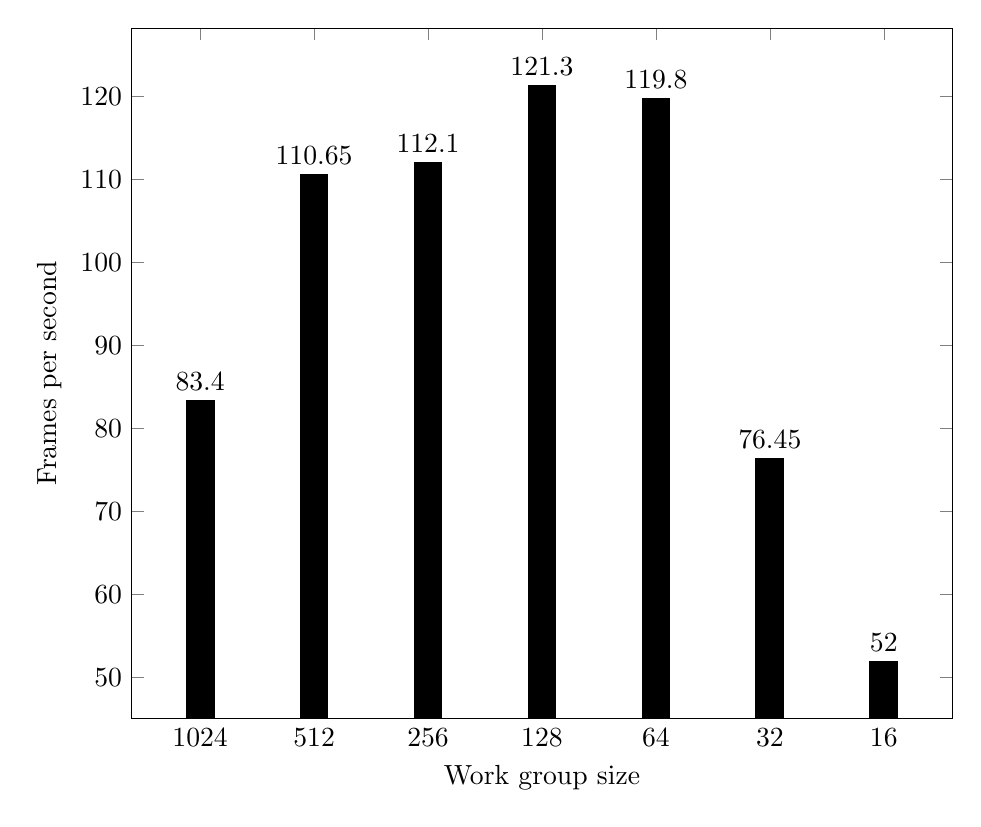
\begin{tikzpicture}
            \begin{axis}
            [
                width=12cm,
                symbolic x coords={1024, 512, 256, 128, 64, 32, 16},
                xtick=data,
                ylabel=Frames per second,
                xlabel=Work group size,
                nodes near coords,
            ]
                \addplot[ybar, fill=black] coordinates
                {
                    (16,52)
                    (32, 76.45)
                    (64, 119.8)
                    (128, 121.3)
                    (256, 112.1)
                    (512, 110.65)
                    (1024, 83.4)
                };
            \end{axis}
        \end{tikzpicture}
        \caption{Frame rates of our 20 000-particle OpenGL implementation between different numbers of work group size}
        \label{fig:work group test}
    \end{figure}
    
\end{doublespace}

\section{Buffers}
\begin{doublespace}
    Buffers are the primary structure to store data on graphics hardware. They represent the GPU's internal memory associated with everything from geometry, textures, and image plane data. From a programming standpoint, an application must initialize the buffers on the GPU that are needed for the application, which is a host-to-device copy operation. Device-to-host copies can be performed as well to pull data from the GPU to the CPU memory \cite[442]{marschner2016}. OpenGL and Vulkan also allow device memory to be mapped into host memory so that an application program can write directly to the buffers on the graphics card. In our implementations, we use a single buffer which stores all the particles state which is used by both the compute pipelines and then reused by the graphics pipeline for rendering.
\end{doublespace}

\section{Shader storage buffer object}

\begin{doublespace}
    A shader storage buffer object (SSBO) is a buffer object that is used to store and retrieve data from within the GLSL. Five SSBOs are used in our implementations, which are bound to a single buffer with different offsets (Listing \ref{lst:buffer offsets in vulkan} and Listing \ref{lst:buffer offsets in opengl}). 
    
    The built-in inputs of compute shaders provide a useful way of accessing elements of a SSBO. For a program that runs through a given number of particles, using \mintinline{glsl}{gl_GlobalInvocation.x} in the shader will give the unique index of a particle.

\end{doublespace}
\begin{longlisting}
\caption{Binding a single buffer to multiple indexed buffer binding points in Vulkan}
\label{lst:buffer offsets in vulkan}
\inputminted[firstline=195, lastline=208]{c++}{code/vulkan.hpp}
\inputminted[firstline=1043, lastline=1070]{c++}{code/vulkan.cpp}
\end{longlisting}

\begin{longlisting}
\caption{Binding a single buffer to multiple indexed buffer binding points in OpenGL}
\label{lst:buffer offsets in opengl}
\inputminted[firstline=249, lastline=262]{c++}{code/opengl.cpp}
\inputminted[firstline=316, lastline=321]{c++}{code/opengl.cpp}
\end{longlisting}

\section{Data dependency and synchronization}

\begin{doublespace}
    % synchronization is an uncountable noun
    Synchronization is the forced ordering of executions, which is important to prevent race conditions. Algorithm \ref{alg:simulation loop} itself has several data dependencies, so it is divided into 3 compute shaders:
    \begin{itemize}
        \item The first reads the position then writes the density and pressure in parallel. It uses data computed by the third compute shader.
        \item The second reads the position, velocity, pressure, and density then writes the force in parallel. It uses data computed by the first compute shader.
        \item And the third reads the force then writes the position and velocity in parallel. It uses data computed by the second compute shader.
    \end{itemize}
    
    Memory barrier and pipeline barrier are used as the synchronization method. They are placed between invocations of compute shaders and between compute and graphics pipeline (Listing \ref{lst:opengl dispatch} and Listing \ref{lst:vulkan dispatch}). This ensures that previous shader has finished writing new data before reading it (read after write [RAW] dependency).
\end{doublespace}

\begin{longlisting}
\caption{Dispatching 3 compute shaders in OpenGL with memory barriers for synchronization}
\label{lst:opengl dispatch}
\begin{minted}[firstnumber=426]{c++}
    glUseProgram(compute_program_handle[0]);
    glDispatchCompute(SPH_NUM_WORK_GROUPS, 1, 1);
    glMemoryBarrier(GL_SHADER_STORAGE_BARRIER_BIT);
    glUseProgram(compute_program_handle[1]);
    glDispatchCompute(SPH_NUM_WORK_GROUPS, 1, 1);
    glMemoryBarrier(GL_SHADER_STORAGE_BARRIER_BIT);
    glUseProgram(compute_program_handle[2]);
    glDispatchCompute(SPH_NUM_WORK_GROUPS, 1, 1);
    glMemoryBarrier(GL_SHADER_STORAGE_BARRIER_BIT);
\end{minted}
\end{longlisting}

\begin{longlisting}
\caption{Dispatching 3 compute shaders in Vulkan with pipeline barriers for synchronization}
\label{lst:vulkan dispatch}
\inputminted[firstline=1253, lastline=1283]{c++}{code/vulkan.cpp}
\end{longlisting}

\section{Simulation parameters}

\begin{doublespace}
The kernel functions are originally designed for 3D, but our implementations are 2D. So the simulation parameters are adjusted to give better results.
\begin{itemize}
    \item particle radius \(r = \SI{0.005}{}\), %meter
    \item initial inter-particle distance \(dx = 2 r\),
    \item particle mass \(m = \SI{0.02}{}\), %\kilo\gram
    \item resting density \(\rho_0 = \SI{1000}{}\), %\kilo\gram\per\cubic\meter
    \item smoothing length \(h = 4 r\),
    \item time step \(dt = \SI{0.001}{}\), %\second
    \item stiffness \(k = \SI{2000}{}\), and % \newton\meter\per\kilo\gram
    \item viscosity \(\mu = \SI{3000}{}\). %\newton\second\per\square\meter
\end{itemize}
\end{doublespace}

\section{Initializing particles}

\begin{doublespace}
    All particles attributes are initialized with 0, and then their locations are set depending on which test case. OpenGL initialize the buffer implicitly by calling \mintinline{c}{glBufferStorage}. In Vulkan, it is done explicitly using a staging buffer. 
\end{doublespace}

\section{Visualization}

\begin{doublespace}
The fluid is visualized as a point cloud. In OpenGL, this is done by simply passing \mintinline{c}{GL_POINTS} to the draw call, while in Vulkan it is done by specifying \mintinline{c}{VK_PRIMITIVE_TOPOLOGY_POINT_LIST} during the graphics pipeline creation.
\end{doublespace}
\chapter{RESULTS}
\label{ch:results}

\section{Test cases}
\begin{doublespace}
    % verification is validation by empirical means. empirical: Based on, concerned with, or verifiable by observation or experience rather than theory or pure logic.
    Two test cases are used to verify that the implementations are correct by examining the visual output. The frame rates of our Vulkan and OpenGL implementations are shown in Figure \ref{fig:particles chart} and Table \ref{table:frame rates}. The first test case is dropping a cube of water inside a box, and the second is a dam break in a closed channel. The water is at rest initially (all velocities zero). The rendering of the first test case and the second test case is shown in Figure \ref{fig:test case 1} and Figure \ref{fig:test case 2} respectively. 
\end{doublespace}

\section{Test environment}
\begin{doublespace}
    Our implementations were tested on a computer with GTX 1070 and i5-6600K at \SI{3.50}{\giga\hertz}, and \SI{16}{\giga\byte} RAM in dual channel. GTX 1070 has \SI{1920} CUDA cores divided into 15 streaming multiprocessors, \SI{98304}{\byte} shared memory per multiprocessor, and \SI{2048} max threads per multiprocessor. The operating system was Windows 10.0.16299.125 64-bit with Visual Studio 2017 15.3.3, Vulkan SDK 1.0.65.1, and NVIDIA video driver 390.77 installed. The third-party libraries used are: OpenGL Mathematics (GLM) 0.9.8.5, The OpenGL Extension Wrangler Library (GLEW) 2.1.0, and GLFW 3.2.1.  % software is mass noun
\end{doublespace}

\section{Performance analysis}
\begin{doublespace}
    Figure \ref{fig:particles chart} shows the implementations' frame rates with different number of particles. The frame rates were obtained from 20 seconds of runtime. Our Vulkan implementation is faster with higher number of particles, but performs worse with lower number of particles.
    
    Our objective is to create real-time simulation, which means the computations must be fast enough that the results can be viewed immediately. Being able to conduct operations at \SI{60}{\hertz} or higher is considered real-time \cite[438]{marschner2016}. So the chosen number of particles is 20 000. The frame rate of our 20 000-particle Vulkan implementation is \SI{115.95}{fps}, and \SI{120.8}{fps} is the frame rate of its OpenGL 4.6 counterpart. 
    
    The OpenGL API statistics from 20-second runtime (00:01 to 00:21) collected using NVIDIA Nsight are shown in Table \ref{table:api time}. The total OpenGL API time is 98.4 \%. Approximately 97.76 \% of time is spent on computation and approximately 0.64 \% is spent on rendering. At the time of writing, NVIDIA Nsight does not support Vulkan profiling, so the statistics for Vulkan are unavailable.
\end{doublespace}

\begin{figure}[H]
    \centering
    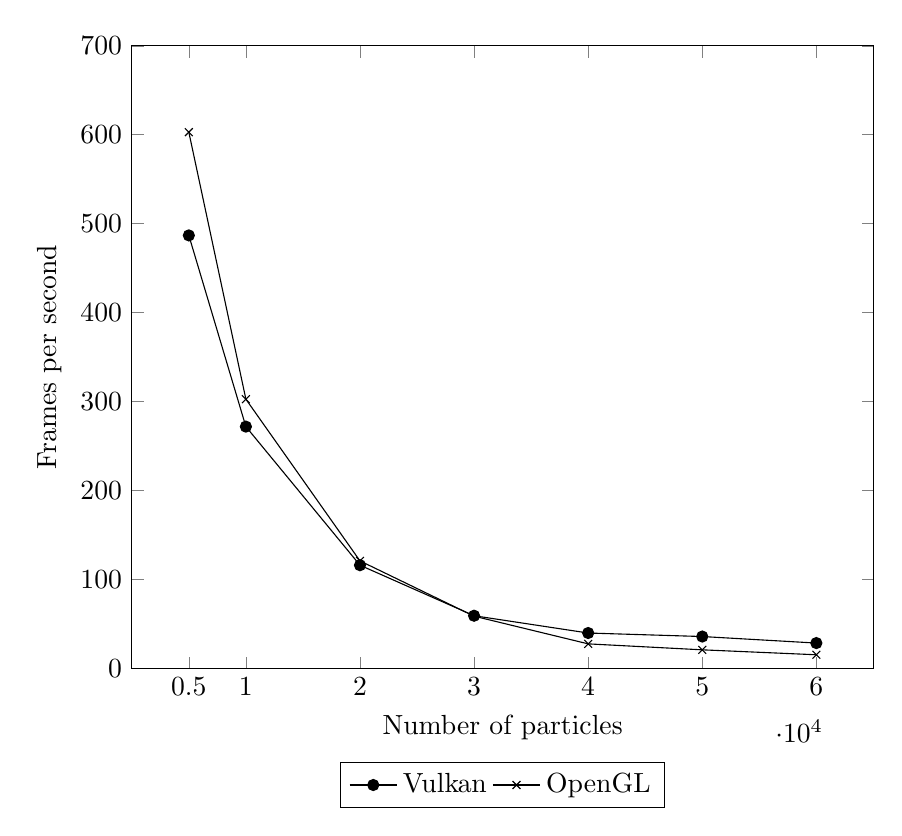
\begin{tikzpicture}
        \begin{axis}
        [
            %title={Vulkan},
            width=11cm,
            legend style={at={(0.5,-0.15)},
            anchor=north,
            legend columns=-1},
            xtick=data,
            xmin=0, xmax=65000,
            ymin=0, ymax=700,
            ylabel=Frames per second,
            xlabel=Number of particles,
        ]
            \addplot[color=black, mark=*] coordinates
            {
                (60000,28.4)
                (50000,35.75)
                (40000,39.7)
                (30000,59.15)
                (20000,115.95)
                (10000,271.8)
                (5000,486.8)
            };
            \addplot[color=black, mark=x] coordinates
            {
                (60000,15.25)
                (50000,20.80)
                (40000,27.5)
                (30000,58.65)
                (20000,120.8)
                (10000,302.65)
                (5000,602.9)
            };
            \legend{Vulkan, OpenGL}
            
        \end{axis}
    \end{tikzpicture}
    \caption{Frame rates comparison}
    \label{fig:particles chart}
\end{figure}


\begin{landscape}

\begin{table}[ht]
    \centering
    \caption{Frame rates table}
    \label{table:frame rates}
    \begin{tabular} {| r | r | r |}
    
        \hline
        \multicolumn{1}{|c|}{\cellcolor{black!10} Number of particles } & \multicolumn{1}{|c|}{\cellcolor{black!10} Vulkan (fps) } & \multicolumn{1}{|c|}{\cellcolor{black!10} OpenGL (fps) } \\ \hline
         5000   &    486.80   &     602.90    \\ \hline
        10000   &    271.80   &     302.65    \\ \hline
        20000   &    115.95   &     120.80    \\ \hline
        30000   &     59.15   &      58.65    \\ \hline
        40000   &     39.70   &      27.50    \\ \hline
        50000   &     35.75   &      20.80    \\ \hline
        60000   &     28.40   &      15.25    \\ \hline
    \end{tabular}
    
    \bigskip
    
    \caption{OpenGL API calls statistics collected from 20 seconds of runtime}
    \label{table:api time}
    \begin{tabular} {| >{\ttfamily}l | r | r | r | r | r | r |}
    
        \hline
        \multicolumn{1}{|c|}{\cellcolor{black!10} Name } & \multicolumn{1}{|c|}{\cellcolor{black!10} Count } & \multicolumn{1}{|c|}{\cellcolor{black!10} Time (\SI{}{\micro\second})) } & \multicolumn{1}{|c|}{\cellcolor{black!10} Time (\%) } & \multicolumn{1}{|c|}{\cellcolor{black!10} Min (\SI{}{\micro\second}) } & \multicolumn{1}{|c|}{\cellcolor{black!10} Avg (\SI{}{\micro\second}) } & \multicolumn{1}{|c|}{\cellcolor{black!10} Max (\SI{}{\micro\second}) }  \\ \hline
        glDispatchCompute & 7539  & 19965136.886    & 95.87  & 2.640    & 2648.247 & 24859.006 \\ \hline
        glMemoryBarrier   & 7539  & 374533.469      & 1.80   & 0.138    & 49.679   & 20221.785 \\ \hline
        glDrawArrays      & 2514  & 67960.646       & 0.33   & 14.054   & 27.032   & 106.307   \\ \hline
        SwapBuffers       & 2514  & 47220.282       & 0.23   & 8.994    & 18.782   & 273.259   \\ \hline
        glUseProgram      & 10054 & 31403.814       & 0.15   & 0.127    & 3.123    & 24811.032 \\ \hline
        GetPixelFormat    & 2514  & 7734.347        & 0.04   & 1.680    & 3.076    & 90.057    \\ \hline
        glClear           & 2514  & 1783.426        & 0.01   & 0.269    & 0.709    & 25.131    \\ \hline
    \end{tabular}
\end{table}

\end{landscape}

%% http://cpp.sh/222ts
\begin{figure}[!ht]
    \minipage{0.245\textwidth}
        \begin{center}
            \includegraphics[width=\linewidth]{images/test_case_1/1.png}
            Frame 1
        \end{center}
    \endminipage
    \hfill
    \minipage{0.245\textwidth}
        \begin{center}
            \includegraphics[width=\linewidth]{images/test_case_1/21.png}
            Frame 21
        \end{center}
    \endminipage
    \hfill
    \minipage{0.245\textwidth}
        \begin{center}
            \includegraphics[width=\linewidth]{images/test_case_1/41.png}
            Frame 41
        \end{center}
    \endminipage
    \hfill
    \minipage{0.245\textwidth}
        \begin{center}
            \includegraphics[width=\linewidth]{images/test_case_1/61.png}
            Frame 61
        \end{center}
    \endminipage
    \hfill

    \addvspace{0.5ex}
    \minipage{0.245\textwidth}
        \begin{center}
            \includegraphics[width=\linewidth]{images/test_case_1/81.png}
            Frame 81
        \end{center}
    \endminipage
    \hfill
    \minipage{0.245\textwidth}
        \begin{center}
            \includegraphics[width=\linewidth]{images/test_case_1/101.png}
            Frame 101
        \end{center}
    \endminipage
    \hfill
    \minipage{0.245\textwidth}
        \begin{center}
            \includegraphics[width=\linewidth]{images/test_case_1/121.png}
            Frame 121
        \end{center}
    \endminipage
    \hfill
    \minipage{0.245\textwidth}
        \begin{center}
            \includegraphics[width=\linewidth]{images/test_case_1/141.png}
            Frame 141
        \end{center}
    \endminipage
    \hfill

    \addvspace{0.5ex}
    \minipage{0.245\textwidth}
        \begin{center}
            \includegraphics[width=\linewidth]{images/test_case_1/161.png}
            Frame 161
        \end{center}
    \endminipage
    \hfill
    \minipage{0.245\textwidth}
        \begin{center}
            \includegraphics[width=\linewidth]{images/test_case_1/181.png}
            Frame 181
        \end{center}
    \endminipage
    \hfill
    \minipage{0.245\textwidth}
        \begin{center}
            \includegraphics[width=\linewidth]{images/test_case_1/201.png}
            Frame 201
        \end{center}
    \endminipage
    \hfill
    \minipage{0.245\textwidth}
        \begin{center}
            \includegraphics[width=\linewidth]{images/test_case_1/221.png}
            Frame 221
        \end{center}
    \endminipage
    \hfill

    \addvspace{0.5ex}
    \minipage{0.245\textwidth}
        \begin{center}
            \includegraphics[width=\linewidth]{images/test_case_1/241.png}
            Frame 241
        \end{center}
    \endminipage
    \hfill
    \minipage{0.245\textwidth}
        \begin{center}
            \includegraphics[width=\linewidth]{images/test_case_1/261.png}
            Frame 261
        \end{center}
    \endminipage
    \hfill
    \minipage{0.245\textwidth}
        \begin{center}
            \includegraphics[width=\linewidth]{images/test_case_1/281.png}
            Frame 281
        \end{center}
    \endminipage
    \hfill
    \minipage{0.245\textwidth}
        \begin{center}
            \includegraphics[width=\linewidth]{images/test_case_1/301.png}
            Frame 301
        \end{center}
    \endminipage
    \hfill

    \addvspace{0.5ex}
    \minipage{0.245\textwidth}
        \begin{center}
            \includegraphics[width=\linewidth]{images/test_case_1/321.png}
            Frame 321
        \end{center}
    \endminipage
    \hfill
    \minipage{0.245\textwidth}
        \begin{center}
            \includegraphics[width=\linewidth]{images/test_case_1/341.png}
            Frame 341
        \end{center}
    \endminipage
    \hfill
    \minipage{0.245\textwidth}
        \begin{center}
            \includegraphics[width=\linewidth]{images/test_case_1/361.png}
            Frame 361
        \end{center}
    \endminipage
    \hfill
    \minipage{0.245\textwidth}
        \begin{center}
            \includegraphics[width=\linewidth]{images/test_case_1/381.png}
            Frame 381
        \end{center}
    \endminipage
    \hfill
\end{figure}
\begin{figure}[!ht]
    \minipage{0.245\textwidth}
        \begin{center}
            \includegraphics[width=\linewidth]{images/test_case_1/401.png}
            Frame 401
        \end{center}
    \endminipage
    \hfill
    \minipage{0.245\textwidth}
        \begin{center}
            \includegraphics[width=\linewidth]{images/test_case_1/421.png}
            Frame 421
        \end{center}
    \endminipage
    \hfill
    \minipage{0.245\textwidth}
        \begin{center}
            \includegraphics[width=\linewidth]{images/test_case_1/441.png}
            Frame 441
        \end{center}
    \endminipage
    \hfill
    \minipage{0.245\textwidth}
        \begin{center}
            \includegraphics[width=\linewidth]{images/test_case_1/461.png}
            Frame 461
        \end{center}
    \endminipage
    \hfill

    \addvspace{0.5ex}
    \minipage{0.245\textwidth}
        \begin{center}
            \includegraphics[width=\linewidth]{images/test_case_1/481.png}
            Frame 481
        \end{center}
    \endminipage
    \hfill
    \minipage{0.245\textwidth}
        \begin{center}
            \includegraphics[width=\linewidth]{images/test_case_1/501.png}
            Frame 501
        \end{center}
    \endminipage
    \hfill
    \minipage{0.245\textwidth}
        \begin{center}
            \includegraphics[width=\linewidth]{images/test_case_1/521.png}
            Frame 521
        \end{center}
    \endminipage
    \hfill
    \minipage{0.245\textwidth}
        \begin{center}
            \includegraphics[width=\linewidth]{images/test_case_1/541.png}
            Frame 541
        \end{center}
    \endminipage
    \hfill

    \addvspace{0.5ex}
    \minipage{0.245\textwidth}
        \begin{center}
            \includegraphics[width=\linewidth]{images/test_case_1/561.png}
            Frame 561
        \end{center}
    \endminipage
    \hfill
    \minipage{0.245\textwidth}
        \begin{center}
            \includegraphics[width=\linewidth]{images/test_case_1/581.png}
            Frame 581
        \end{center}
    \endminipage
    \hfill
    \minipage{0.245\textwidth}
        \begin{center}
            \includegraphics[width=\linewidth]{images/test_case_1/601.png}
            Frame 601
        \end{center}
    \endminipage
    \hfill
    \minipage{0.245\textwidth}
        \begin{center}
            \includegraphics[width=\linewidth]{images/test_case_1/621.png}
            Frame 621
        \end{center}
    \endminipage
    \hfill

    \addvspace{0.5ex}
    \minipage{0.245\textwidth}
        \begin{center}
            \includegraphics[width=\linewidth]{images/test_case_1/641.png}
            Frame 641
        \end{center}
    \endminipage
    \hfill
    \minipage{0.245\textwidth}
        \begin{center}
            \includegraphics[width=\linewidth]{images/test_case_1/661.png}
            Frame 661
        \end{center}
    \endminipage
    \hfill
    \minipage{0.245\textwidth}
        \begin{center}
            \includegraphics[width=\linewidth]{images/test_case_1/681.png}
            Frame 681
        \end{center}
    \endminipage
    \hfill
    \minipage{0.245\textwidth}
        \begin{center}
            \includegraphics[width=\linewidth]{images/test_case_1/701.png}
            Frame 701
        \end{center}
    \endminipage
    \hfill

    \addvspace{0.5ex}
    \minipage{0.245\textwidth}
        \begin{center}
            \includegraphics[width=\linewidth]{images/test_case_1/721.png}
            Frame 721
        \end{center}
    \endminipage
    \hfill
    \minipage{0.245\textwidth}
        \begin{center}
            \includegraphics[width=\linewidth]{images/test_case_1/741.png}
            Frame 741
        \end{center}
    \endminipage
    \hfill
    \minipage{0.245\textwidth}
        \begin{center}
            \includegraphics[width=\linewidth]{images/test_case_1/761.png}
            Frame 761
        \end{center}
    \endminipage
    \hfill
    \minipage{0.245\textwidth}
        \begin{center}
            \includegraphics[width=\linewidth]{images/test_case_1/781.png}
            Frame 781
        \end{center}
    \endminipage
    \hfill
\end{figure}
\begin{figure}[!ht]
    \minipage{0.245\textwidth}
        \begin{center}
            \includegraphics[width=\linewidth]{images/test_case_1/801.png}
            Frame 801
        \end{center}
    \endminipage
    \hfill
    \minipage{0.245\textwidth}
        \begin{center}
            \includegraphics[width=\linewidth]{images/test_case_1/821.png}
            Frame 821
        \end{center}
    \endminipage
    \hfill
    \minipage{0.245\textwidth}
        \begin{center}
            \includegraphics[width=\linewidth]{images/test_case_1/841.png}
            Frame 841
        \end{center}
    \endminipage
    \hfill
    \minipage{0.245\textwidth}
        \begin{center}
            \includegraphics[width=\linewidth]{images/test_case_1/861.png}
            Frame 861
        \end{center}
    \endminipage
    \hfill

    \addvspace{0.5ex}
    \minipage{0.245\textwidth}
        \begin{center}
            \includegraphics[width=\linewidth]{images/test_case_1/881.png}
            Frame 881
        \end{center}
    \endminipage
    \hfill
    \minipage{0.245\textwidth}
        \begin{center}
            \includegraphics[width=\linewidth]{images/test_case_1/901.png}
            Frame 901
        \end{center}
    \endminipage
    \hfill
    \minipage{0.245\textwidth}
        \begin{center}
            \includegraphics[width=\linewidth]{images/test_case_1/921.png}
            Frame 921
        \end{center}
    \endminipage
    \hfill
    \minipage{0.245\textwidth}
        \begin{center}
            \includegraphics[width=\linewidth]{images/test_case_1/941.png}
            Frame 941
        \end{center}
    \endminipage
    \hfill

    \addvspace{0.5ex}
    \minipage{0.245\textwidth}
        \begin{center}
            \includegraphics[width=\linewidth]{images/test_case_1/961.png}
            Frame 961
        \end{center}
    \endminipage
    \hfill
    \minipage{0.245\textwidth}
        \begin{center}
            \includegraphics[width=\linewidth]{images/test_case_1/981.png}
            Frame 981
        \end{center}
    \endminipage
    \hfill
    \minipage{0.245\textwidth}
        \begin{center}
            \includegraphics[width=\linewidth]{images/test_case_1/1001.png}
            Frame 1001
        \end{center}
    \endminipage
    \hfill
    \minipage{0.245\textwidth}
        \begin{center}
            \includegraphics[width=\linewidth]{images/test_case_1/1021.png}
            Frame 1021
        \end{center}
    \endminipage
    \hfill

    \addvspace{0.5ex}
    \minipage{0.245\textwidth}
        \begin{center}
            \includegraphics[width=\linewidth]{images/test_case_1/1041.png}
            Frame 1041
        \end{center}
    \endminipage
    \hfill
    \minipage{0.245\textwidth}
        \begin{center}
            \includegraphics[width=\linewidth]{images/test_case_1/1061.png}
            Frame 1061
        \end{center}
    \endminipage
    \hfill
    \minipage{0.245\textwidth}
        \begin{center}
            \includegraphics[width=\linewidth]{images/test_case_1/1081.png}
            Frame 1081
        \end{center}
    \endminipage
    \hfill
    \minipage{0.245\textwidth}
        \begin{center}
            \includegraphics[width=\linewidth]{images/test_case_1/1101.png}
            Frame 1101
        \end{center}
    \endminipage
    \hfill

    \addvspace{0.5ex}
    \minipage{0.245\textwidth}
        \begin{center}
            \includegraphics[width=\linewidth]{images/test_case_1/1121.png}
            Frame 1121
        \end{center}
    \endminipage
    \hfill
    \minipage{0.245\textwidth}
        \begin{center}
            \includegraphics[width=\linewidth]{images/test_case_1/1141.png}
            Frame 1141
        \end{center}
    \endminipage
    \hfill
    \minipage{0.245\textwidth}
        \begin{center}
            \includegraphics[width=\linewidth]{images/test_case_1/1161.png}
            Frame 1161
        \end{center}
    \endminipage
    \hfill
    \minipage{0.245\textwidth}
        \begin{center}
            \includegraphics[width=\linewidth]{images/test_case_1/1181.png}
            Frame 1181
        \end{center}
    \endminipage
    \hfill
\end{figure}
\begin{figure}[!ht]
    \minipage{0.245\textwidth}
        \begin{center}
            \includegraphics[width=\linewidth]{images/test_case_1/1201.png}
            Frame 1201
        \end{center}
    \endminipage
    \hfill
    \minipage{0.245\textwidth}
        \begin{center}
            \includegraphics[width=\linewidth]{images/test_case_1/1221.png}
            Frame 1221
        \end{center}
    \endminipage
    \hfill
    \minipage{0.245\textwidth}
        \begin{center}
            \includegraphics[width=\linewidth]{images/test_case_1/1241.png}
            Frame 1241
        \end{center}
    \endminipage
    \hfill
    \minipage{0.245\textwidth}
        \begin{center}
            \includegraphics[width=\linewidth]{images/test_case_1/1261.png}
            Frame 1261
        \end{center}
    \endminipage
    \hfill

    \addvspace{0.5ex}
    \minipage{0.245\textwidth}
        \begin{center}
            \includegraphics[width=\linewidth]{images/test_case_1/1281.png}
            Frame 1281
        \end{center}
    \endminipage
    \hfill
    \minipage{0.245\textwidth}
        \begin{center}
            \includegraphics[width=\linewidth]{images/test_case_1/1301.png}
            Frame 1301
        \end{center}
    \endminipage
    \hfill
    \minipage{0.245\textwidth}
        \begin{center}
            \includegraphics[width=\linewidth]{images/test_case_1/1321.png}
            Frame 1321
        \end{center}
    \endminipage
    \hfill
    \minipage{0.245\textwidth}
        \begin{center}
            \includegraphics[width=\linewidth]{images/test_case_1/1341.png}
            Frame 1341
        \end{center}
    \endminipage
    \hfill

    \addvspace{0.5ex}
    \minipage{0.245\textwidth}
        \begin{center}
            \includegraphics[width=\linewidth]{images/test_case_1/1361.png}
            Frame 1361
        \end{center}
    \endminipage
    \hfill
    \minipage{0.245\textwidth}
        \begin{center}
            \includegraphics[width=\linewidth]{images/test_case_1/1381.png}
            Frame 1381
        \end{center}
    \endminipage
    \hfill
    \minipage{0.245\textwidth}
        \begin{center}
            \includegraphics[width=\linewidth]{images/test_case_1/1401.png}
            Frame 1401
        \end{center}
    \endminipage
    \hfill
    \minipage{0.245\textwidth}
        \begin{center}
            \includegraphics[width=\linewidth]{images/test_case_1/1421.png}
            Frame 1421
        \end{center}
    \endminipage
    \hfill

    \addvspace{0.5ex}
    \minipage{0.245\textwidth}
        \begin{center}
            \includegraphics[width=\linewidth]{images/test_case_1/1441.png}
            Frame 1441
        \end{center}
    \endminipage
    \hfill
    \minipage{0.245\textwidth}
        \begin{center}
            \includegraphics[width=\linewidth]{images/test_case_1/1461.png}
            Frame 1461
        \end{center}
    \endminipage
    \hfill
    \minipage{0.245\textwidth}
        \begin{center}
            \includegraphics[width=\linewidth]{images/test_case_1/1481.png}
            Frame 1481
        \end{center}
    \endminipage
    \hfill
    \minipage{0.245\textwidth}
        \begin{center}
            \includegraphics[width=\linewidth]{images/test_case_1/1501.png}
            Frame 1501
        \end{center}
    \endminipage
    \hfill

    \addvspace{0.5ex}
    \minipage{0.245\textwidth}
        \begin{center}
            \includegraphics[width=\linewidth]{images/test_case_1/1521.png}
            Frame 1521
        \end{center}
    \endminipage
    \hfill
    \minipage{0.245\textwidth}
        \begin{center}
            \includegraphics[width=\linewidth]{images/test_case_1/1541.png}
            Frame 1541
        \end{center}
    \endminipage
    \hfill
    \minipage{0.245\textwidth}
        \begin{center}
            \includegraphics[width=\linewidth]{images/test_case_1/1561.png}
            Frame 1561
        \end{center}
    \endminipage
    \hfill
    \minipage{0.245\textwidth}
        \begin{center}
            \includegraphics[width=\linewidth]{images/test_case_1/1581.png}
            Frame 1581
        \end{center}
    \endminipage
    \hfill

    \caption{Rendering of the first test case}
    \label{fig:test case 1}
\end{figure}

\begin{figure}[!ht]
    \minipage{0.245\textwidth}
        \begin{center}
            \includegraphics[width=\linewidth]{images/test_case_2/1.png}
            Frame 1
        \end{center}
    \endminipage
    \hfill
    \minipage{0.245\textwidth}
        \begin{center}
            \includegraphics[width=\linewidth]{images/test_case_2/21.png}
            Frame 21
        \end{center}
    \endminipage
    \hfill
    \minipage{0.245\textwidth}
        \begin{center}
            \includegraphics[width=\linewidth]{images/test_case_2/41.png}
            Frame 41
        \end{center}
    \endminipage
    \hfill
    \minipage{0.245\textwidth}
        \begin{center}
            \includegraphics[width=\linewidth]{images/test_case_2/61.png}
            Frame 61
        \end{center}
    \endminipage
    \hfill

    \addvspace{0.5ex}
    \minipage{0.245\textwidth}
        \begin{center}
            \includegraphics[width=\linewidth]{images/test_case_2/81.png}
            Frame 81
        \end{center}
    \endminipage
    \hfill
    \minipage{0.245\textwidth}
        \begin{center}
            \includegraphics[width=\linewidth]{images/test_case_2/101.png}
            Frame 101
        \end{center}
    \endminipage
    \hfill
    \minipage{0.245\textwidth}
        \begin{center}
            \includegraphics[width=\linewidth]{images/test_case_2/121.png}
            Frame 121
        \end{center}
    \endminipage
    \hfill
    \minipage{0.245\textwidth}
        \begin{center}
            \includegraphics[width=\linewidth]{images/test_case_2/141.png}
            Frame 141
        \end{center}
    \endminipage
    \hfill

    \addvspace{0.5ex}
    \minipage{0.245\textwidth}
        \begin{center}
            \includegraphics[width=\linewidth]{images/test_case_2/161.png}
            Frame 161
        \end{center}
    \endminipage
    \hfill
    \minipage{0.245\textwidth}
        \begin{center}
            \includegraphics[width=\linewidth]{images/test_case_2/181.png}
            Frame 181
        \end{center}
    \endminipage
    \hfill
    \minipage{0.245\textwidth}
        \begin{center}
            \includegraphics[width=\linewidth]{images/test_case_2/201.png}
            Frame 201
        \end{center}
    \endminipage
    \hfill
    \minipage{0.245\textwidth}
        \begin{center}
            \includegraphics[width=\linewidth]{images/test_case_2/221.png}
            Frame 221
        \end{center}
    \endminipage
    \hfill

    \addvspace{0.5ex}
    \minipage{0.245\textwidth}
        \begin{center}
            \includegraphics[width=\linewidth]{images/test_case_2/241.png}
            Frame 241
        \end{center}
    \endminipage
    \hfill
    \minipage{0.245\textwidth}
        \begin{center}
            \includegraphics[width=\linewidth]{images/test_case_2/261.png}
            Frame 261
        \end{center}
    \endminipage
    \hfill
    \minipage{0.245\textwidth}
        \begin{center}
            \includegraphics[width=\linewidth]{images/test_case_2/281.png}
            Frame 281
        \end{center}
    \endminipage
    \hfill
    \minipage{0.245\textwidth}
        \begin{center}
            \includegraphics[width=\linewidth]{images/test_case_2/301.png}
            Frame 301
        \end{center}
    \endminipage
    \hfill

    \addvspace{0.5ex}
    \minipage{0.245\textwidth}
        \begin{center}
            \includegraphics[width=\linewidth]{images/test_case_2/321.png}
            Frame 321
        \end{center}
    \endminipage
    \hfill
    \minipage{0.245\textwidth}
        \begin{center}
            \includegraphics[width=\linewidth]{images/test_case_2/341.png}
            Frame 341
        \end{center}
    \endminipage
    \hfill
    \minipage{0.245\textwidth}
        \begin{center}
            \includegraphics[width=\linewidth]{images/test_case_2/361.png}
            Frame 361
        \end{center}
    \endminipage
    \hfill
    \minipage{0.245\textwidth}
        \begin{center}
            \includegraphics[width=\linewidth]{images/test_case_2/381.png}
            Frame 381
        \end{center}
    \endminipage
    \hfill
\end{figure}
\begin{figure}[!ht]
    \minipage{0.245\textwidth}
        \begin{center}
            \includegraphics[width=\linewidth]{images/test_case_2/401.png}
            Frame 401
        \end{center}
    \endminipage
    \hfill
    \minipage{0.245\textwidth}
        \begin{center}
            \includegraphics[width=\linewidth]{images/test_case_2/421.png}
            Frame 421
        \end{center}
    \endminipage
    \hfill
    \minipage{0.245\textwidth}
        \begin{center}
            \includegraphics[width=\linewidth]{images/test_case_2/441.png}
            Frame 441
        \end{center}
    \endminipage
    \hfill
    \minipage{0.245\textwidth}
        \begin{center}
            \includegraphics[width=\linewidth]{images/test_case_2/461.png}
            Frame 461
        \end{center}
    \endminipage
    \hfill

    \addvspace{0.5ex}
    \minipage{0.245\textwidth}
        \begin{center}
            \includegraphics[width=\linewidth]{images/test_case_2/481.png}
            Frame 481
        \end{center}
    \endminipage
    \hfill
    \minipage{0.245\textwidth}
        \begin{center}
            \includegraphics[width=\linewidth]{images/test_case_2/501.png}
            Frame 501
        \end{center}
    \endminipage
    \hfill
    \minipage{0.245\textwidth}
        \begin{center}
            \includegraphics[width=\linewidth]{images/test_case_2/521.png}
            Frame 521
        \end{center}
    \endminipage
    \hfill
    \minipage{0.245\textwidth}
        \begin{center}
            \includegraphics[width=\linewidth]{images/test_case_2/541.png}
            Frame 541
        \end{center}
    \endminipage
    \hfill

    \addvspace{0.5ex}
    \minipage{0.245\textwidth}
        \begin{center}
            \includegraphics[width=\linewidth]{images/test_case_2/561.png}
            Frame 561
        \end{center}
    \endminipage
    \hfill
    \minipage{0.245\textwidth}
        \begin{center}
            \includegraphics[width=\linewidth]{images/test_case_2/581.png}
            Frame 581
        \end{center}
    \endminipage
    \hfill
    \minipage{0.245\textwidth}
        \begin{center}
            \includegraphics[width=\linewidth]{images/test_case_2/601.png}
            Frame 601
        \end{center}
    \endminipage
    \hfill
    \minipage{0.245\textwidth}
        \begin{center}
            \includegraphics[width=\linewidth]{images/test_case_2/621.png}
            Frame 621
        \end{center}
    \endminipage
    \hfill

    \addvspace{0.5ex}
    \minipage{0.245\textwidth}
        \begin{center}
            \includegraphics[width=\linewidth]{images/test_case_2/641.png}
            Frame 641
        \end{center}
    \endminipage
    \hfill
    \minipage{0.245\textwidth}
        \begin{center}
            \includegraphics[width=\linewidth]{images/test_case_2/661.png}
            Frame 661
        \end{center}
    \endminipage
    \hfill
    \minipage{0.245\textwidth}
        \begin{center}
            \includegraphics[width=\linewidth]{images/test_case_2/681.png}
            Frame 681
        \end{center}
    \endminipage
    \hfill
    \minipage{0.245\textwidth}
        \begin{center}
            \includegraphics[width=\linewidth]{images/test_case_2/701.png}
            Frame 701
        \end{center}
    \endminipage
    \hfill

    \addvspace{0.5ex}
    \minipage{0.245\textwidth}
        \begin{center}
            \includegraphics[width=\linewidth]{images/test_case_2/721.png}
            Frame 721
        \end{center}
    \endminipage
    \hfill
    \minipage{0.245\textwidth}
        \begin{center}
            \includegraphics[width=\linewidth]{images/test_case_2/741.png}
            Frame 741
        \end{center}
    \endminipage
    \hfill
    \minipage{0.245\textwidth}
        \begin{center}
            \includegraphics[width=\linewidth]{images/test_case_2/761.png}
            Frame 761
        \end{center}
    \endminipage
    \hfill
    \minipage{0.245\textwidth}
        \begin{center}
            \includegraphics[width=\linewidth]{images/test_case_2/781.png}
            Frame 781
        \end{center}
    \endminipage
    \hfill
\end{figure}
\begin{figure}[!ht]
    \minipage{0.245\textwidth}
        \begin{center}
            \includegraphics[width=\linewidth]{images/test_case_2/801.png}
            Frame 801
        \end{center}
    \endminipage
    \hfill
    \minipage{0.245\textwidth}
        \begin{center}
            \includegraphics[width=\linewidth]{images/test_case_2/821.png}
            Frame 821
        \end{center}
    \endminipage
    \hfill
    \minipage{0.245\textwidth}
        \begin{center}
            \includegraphics[width=\linewidth]{images/test_case_2/841.png}
            Frame 841
        \end{center}
    \endminipage
    \hfill
    \minipage{0.245\textwidth}
        \begin{center}
            \includegraphics[width=\linewidth]{images/test_case_2/861.png}
            Frame 861
        \end{center}
    \endminipage
    \hfill

    \addvspace{0.5ex}
    \minipage{0.245\textwidth}
        \begin{center}
            \includegraphics[width=\linewidth]{images/test_case_2/881.png}
            Frame 881
        \end{center}
    \endminipage
    \hfill
    \minipage{0.245\textwidth}
        \begin{center}
            \includegraphics[width=\linewidth]{images/test_case_2/901.png}
            Frame 901
        \end{center}
    \endminipage
    \hfill
    \minipage{0.245\textwidth}
        \begin{center}
            \includegraphics[width=\linewidth]{images/test_case_2/921.png}
            Frame 921
        \end{center}
    \endminipage
    \hfill
    \minipage{0.245\textwidth}
        \begin{center}
            \includegraphics[width=\linewidth]{images/test_case_2/941.png}
            Frame 941
        \end{center}
    \endminipage
    \hfill

    \addvspace{0.5ex}
    \minipage{0.245\textwidth}
        \begin{center}
            \includegraphics[width=\linewidth]{images/test_case_2/961.png}
            Frame 961
        \end{center}
    \endminipage
    \hfill
    \minipage{0.245\textwidth}
        \begin{center}
            \includegraphics[width=\linewidth]{images/test_case_2/981.png}
            Frame 981
        \end{center}
    \endminipage
    \hfill
    \minipage{0.245\textwidth}
        \begin{center}
            \includegraphics[width=\linewidth]{images/test_case_2/1001.png}
            Frame 1001
        \end{center}
    \endminipage
    \hfill
    \minipage{0.245\textwidth}
        \begin{center}
            \includegraphics[width=\linewidth]{images/test_case_2/1021.png}
            Frame 1021
        \end{center}
    \endminipage
    \hfill

    \addvspace{0.5ex}
    \minipage{0.245\textwidth}
        \begin{center}
            \includegraphics[width=\linewidth]{images/test_case_2/1041.png}
            Frame 1041
        \end{center}
    \endminipage
    \hfill
    \minipage{0.245\textwidth}
        \begin{center}
            \includegraphics[width=\linewidth]{images/test_case_2/1061.png}
            Frame 1061
        \end{center}
    \endminipage
    \hfill
    \minipage{0.245\textwidth}
        \begin{center}
            \includegraphics[width=\linewidth]{images/test_case_2/1081.png}
            Frame 1081
        \end{center}
    \endminipage
    \hfill
    \minipage{0.245\textwidth}
        \begin{center}
            \includegraphics[width=\linewidth]{images/test_case_2/1101.png}
            Frame 1101
        \end{center}
    \endminipage
    \hfill

    \addvspace{0.5ex}
    \minipage{0.245\textwidth}
        \begin{center}
            \includegraphics[width=\linewidth]{images/test_case_2/1121.png}
            Frame 1121
        \end{center}
    \endminipage
    \hfill
    \minipage{0.245\textwidth}
        \begin{center}
            \includegraphics[width=\linewidth]{images/test_case_2/1141.png}
            Frame 1141
        \end{center}
    \endminipage
    \hfill
    \minipage{0.245\textwidth}
        \begin{center}
            \includegraphics[width=\linewidth]{images/test_case_2/1161.png}
            Frame 1161
        \end{center}
    \endminipage
    \hfill
    \minipage{0.245\textwidth}
        \begin{center}
            \includegraphics[width=\linewidth]{images/test_case_2/1181.png}
            Frame 1181
        \end{center}
    \endminipage
    \hfill
\end{figure}
\begin{figure}[!ht]
    \minipage{0.245\textwidth}
        \begin{center}
            \includegraphics[width=\linewidth]{images/test_case_2/1201.png}
            Frame 1201
        \end{center}
    \endminipage
    \hfill
    \minipage{0.245\textwidth}
        \begin{center}
            \includegraphics[width=\linewidth]{images/test_case_2/1221.png}
            Frame 1221
        \end{center}
    \endminipage
    \hfill
    \minipage{0.245\textwidth}
        \begin{center}
            \includegraphics[width=\linewidth]{images/test_case_2/1241.png}
            Frame 1241
        \end{center}
    \endminipage
    \hfill
    \minipage{0.245\textwidth}
        \begin{center}
            \includegraphics[width=\linewidth]{images/test_case_2/1261.png}
            Frame 1261
        \end{center}
    \endminipage
    \hfill

    \addvspace{0.5ex}
    \minipage{0.245\textwidth}
        \begin{center}
            \includegraphics[width=\linewidth]{images/test_case_2/1281.png}
            Frame 1281
        \end{center}
    \endminipage
    \hfill
    \minipage{0.245\textwidth}
        \begin{center}
            \includegraphics[width=\linewidth]{images/test_case_2/1301.png}
            Frame 1301
        \end{center}
    \endminipage
    \hfill
    \minipage{0.245\textwidth}
        \begin{center}
            \includegraphics[width=\linewidth]{images/test_case_2/1321.png}
            Frame 1321
        \end{center}
    \endminipage
    \hfill
    \minipage{0.245\textwidth}
        \begin{center}
            \includegraphics[width=\linewidth]{images/test_case_2/1341.png}
            Frame 1341
        \end{center}
    \endminipage
    \hfill

    \addvspace{0.5ex}
    \minipage{0.245\textwidth}
        \begin{center}
            \includegraphics[width=\linewidth]{images/test_case_2/1361.png}
            Frame 1361
        \end{center}
    \endminipage
    \hfill
    \minipage{0.245\textwidth}
        \begin{center}
            \includegraphics[width=\linewidth]{images/test_case_2/1381.png}
            Frame 1381
        \end{center}
    \endminipage
    \hfill
    \minipage{0.245\textwidth}
        \begin{center}
            \includegraphics[width=\linewidth]{images/test_case_2/1401.png}
            Frame 1401
        \end{center}
    \endminipage
    \hfill
    \minipage{0.245\textwidth}
        \begin{center}
            \includegraphics[width=\linewidth]{images/test_case_2/1421.png}
            Frame 1421
        \end{center}
    \endminipage
    \hfill

    \addvspace{0.5ex}
    \minipage{0.245\textwidth}
        \begin{center}
            \includegraphics[width=\linewidth]{images/test_case_2/1441.png}
            Frame 1441
        \end{center}
    \endminipage
    \hfill
    \minipage{0.245\textwidth}
        \begin{center}
            \includegraphics[width=\linewidth]{images/test_case_2/1461.png}
            Frame 1461
        \end{center}
    \endminipage
    \hfill
    \minipage{0.245\textwidth}
        \begin{center}
            \includegraphics[width=\linewidth]{images/test_case_2/1481.png}
            Frame 1481
        \end{center}
    \endminipage
    \hfill
    \minipage{0.245\textwidth}
        \begin{center}
            \includegraphics[width=\linewidth]{images/test_case_2/1501.png}
            Frame 1501
        \end{center}
    \endminipage
    \hfill

    \addvspace{0.5ex}
    \minipage{0.245\textwidth}
        \begin{center}
            \includegraphics[width=\linewidth]{images/test_case_2/1521.png}
            Frame 1521
        \end{center}
    \endminipage
    \hfill
    \minipage{0.245\textwidth}
        \begin{center}
            \includegraphics[width=\linewidth]{images/test_case_2/1541.png}
            Frame 1541
        \end{center}
    \endminipage
    \hfill
    \minipage{0.245\textwidth}
        \begin{center}
            \includegraphics[width=\linewidth]{images/test_case_2/1561.png}
            Frame 1561
        \end{center}
    \endminipage
    \hfill
    \minipage{0.245\textwidth}
        \begin{center}
            \includegraphics[width=\linewidth]{images/test_case_2/1581.png}
            Frame 1581
        \end{center}
    \endminipage
    \hfill

    \caption{Rendering of the second test case}
    \label{fig:test case 2}
\end{figure}

\chapter{CONCLUSIONS}
\label{ch:conclusions}

\begin{doublespace}
    In this thesis, we investigate the potential of Vulkan for fluid animation using SPH method. We begin by devising a simple parallel SPH algorithm. Then we implement this algorithm in GLSL compute shader. Then we proceed to develop Vulkan and OpenGL implementations which use the same GLSL code in SPIR-V format. With 2 test cases, we verify that the implementations are correct by examining the visual output, and then measure its performance.
    
    If the number of particles is 30 000 or greater, our Vulkan implementation performs faster compared to our OpenGL implementation. But our Vulkan implementation  performs worse compared to our OpenGL implementation if the number of particles is 20 000 or fewer.
\end{doublespace}

\printbibliography[title={BIBLIOGRAPHY}, heading=bibintoc]

%%
 % Appendices
 %%
\begin{appendices}

\renewcommand{\thelisting}{\Alph{chapter}.\arabic{listing}}

\addtocontents{toc}{\string\let\string\chaporappname\string\appendixname}

\pretocmd{\chapter}
{
  \clearpage
  \pagenumbering{arabic}
  \renewcommand*{\thepage}{\thechapter\arabic{page}}
}{}{}

\chapter{COMPLETE GLSL LISTINGS}
\label{ch:glsl}

\begin{longlisting}
\caption{Compute shader 1---compute density and pressure}
\label{lst:stage 1}
\inputminted[]{glsl}{code/1.comp}
\end{longlisting}

\begin{longlisting}
\caption{Compute shader 2---compute forces}
\label{lst:stage 2}
\inputminted[]{glsl}{code/2.comp}
\end{longlisting}

\begin{longlisting}
\caption{Compute shader 3---integrate and handle collision with the edges}
\label{lst:stage 3}
\inputminted[]{glsl}{code/3.comp}
\end{longlisting}

\begin{longlisting}
\caption{Vertex shader}
\label{lst:vertex shader}
\inputminted[]{glsl}{code/particle.vert}
\end{longlisting}

\begin{longlisting}
\caption{Fragment shader}
\label{lst:fragment shader}
\inputminted[]{glsl}{code/particle.frag}
\end{longlisting}

\clearpage

\end{appendices}

\backmatter

\end{document}
